\documentclass[sigconf, review, anonymous]{acmart} %timestamp 
% \documentclass[sigconf, review]{acmart} %timestamp 
%, timestamp
%\usepackage{usenix}
%end of changed lines
%\usepackage{times}
%\usepackage{microtype}
%\usepackage[hyphens]{url} %Option clash
\usepackage{amsmath, amssymb, amsfonts, mathrsfs}
\usepackage{balance}
\usepackage{leading}
\usepackage{graphicx}
\usepackage{subfig}
%Removing the geometry package used for Tighter Format
%\usepackage{geometry}
%\usepackage{times}
\usepackage{textcomp}
\usepackage{multirow}
\usepackage{framed}
\usepackage{amsmath}
\usepackage{listings}
\usepackage{xspace}
\usepackage{enumitem}
\usepackage{microtype}
%\usepackage{hyperref}
%\usepackage[usenames,dvipsnames,svgnames,table]{xcolor} %Option Clash
%\usepackage[lined,noend,linesnumbered]{algorithm2e}
\usepackage{cleveref}

%%% Local Variables:
%%% mode: latex
%%% TeX-master: "paper"
%%% End:


\crefformat{section}{\S#2#1#3} % see manual of cleveref, section 8.2.1

\newcommand{\sysname}{SciSpot\xspace}

%\newcommand{\comment}[1]{{\color{blue}[\textsf{#1}]}}

%\newcommand{\TODO}[1]{\comment{TODO: #1}}
%\renewcommand{\paragraph}[1]{\textbf{#1}}


\RequirePackage[normalem]{ulem}
\RequirePackage{color}\definecolor{RED}{rgb}{1,0,0}\definecolor{BLUE}{rgb}{0,0,1}
\providecommand{\DIFadd}[1]{{\protect\color{blue}\uwave{#1}}}
\providecommand{\DIFdel}[1]{{\protect\color{red}\sout{#1}}}
%DIF SAFE PREAMBLE
\providecommand{\DIFaddbegin}{}
\providecommand{\DIFaddend}{}
\providecommand{\DIFdelbegin}{}
\providecommand{\DIFdelend}{}
%DIF FLOATSAFE PREAMBLE
\providecommand{\DIFaddFL}[1]{\DIFadd{#1}}
\providecommand{\DIFdelFL}[1]{\DIFdel{#1}}
\providecommand{\DIFaddbeginFL}{}
\providecommand{\DIFaddendFL}{}
\providecommand{\DIFdelbeginFL}{}
\providecommand{\DIFdelendFL}{}
%DIF END PREAMBLE EXTENSION ADDED BY LATEXDIFF

\def\Section {\S}

\newcommand{\squishlist}{
 \begin{list}{$\bullet$}
  { \setlength{\itemsep}{0pt}
     \setlength{\parsep}{3pt}
     \setlength{\topsep}{3pt}
     \setlength{\partopsep}{0pt}
     \setlength{\leftmargin}{1.5em}
     \setlength{\labelwidth}{1em}
     \setlength{\labelsep}{0.5em} } }
	
\newcommand{\squishlisttwo}{
 \begin{list}{$\bullet$}
  { \setlength{\itemsep}{0pt}
     \setlength{\parsep}{0pt}
    \setlength{\topsep}{0pt}
    \setlength{\partopsep}{0pt}
    \setlength{\leftmargin}{2em}
    \setlength{\labelwidth}{1.5em}
    \setlength{\labelsep}{0.5em} } }

\newcommand{\squishend}{
  \end{list}  }

\newcommand{\alert}[1] {\textcolor{red} {\textsc{#1}}}

\newcommand{\myfbox}[1] {\noindent \fbox{\parbox{0.5\textwidth} {#1}}}

\newcommand{\mhead}[1] {\noindent \textbf{#1}}

\newcommand*\mean[1]{\overline{#1}}

\newcommand{\eat}[1]{}

\newcommand{\compresslist}{%
  \setlength{\itemsep}{1pt}%
  \setlength{\leftmargin}{1.5em}
  \setlength{\labelwidth}{1em}
  \setlength{\parskip}{0pt}%
  \setlength{\parsep}{0pt}%
%  \setlength{\itemindent}{-10pt}%
}

\newcommand{\myfigspace}[0]{-0.45cm}
\newcommand{\bigfigspace}[0]{-0.9cm}
\newcommand{\captionspace}[0]{-0.5cm}
\newcommand{\subsecspace}[0]{-0.33cm}
\newcommand{\largesubsecspace}[0]{-0.40cm}
\newcommand{\tightext}[0]{-0.12cm}
\newcommand{\eqnspace}[0]{-0.1cm}

%%% Local Variables:
%%% mode: latex
%%% TeX-master: "paper"
%%% End:


\newcommand{\sign}[1]{\operatorname{sign}\left({#1}\right)}


\newcommand\prat[1]{\noindent \textcolor{red}{(Prateek: #1)}}
\newcommand\vikram[1]{\textcolor{blue}{(Vikram: #1)}}
%\newcommand\vj[1]{\textcolor{blue}{#1}} %for inline smaller changes

%%%%%%%% For submission only

\setcopyright{none}
\settopmatter{printacmref=false}
\acmConference{}{}{}
\acmPrice{}
\acmISBN{}
\acmDOI{}
\acmYear{}
\acmMonth{}
\settopmatter{printfolios=true}
%%%%%%%%%%%%%%%%%%%

\raggedbottom

\begin{document}
% \title{SciSpot: A Framework for Low-cost Scientific Computing On Transient Cloud Servers}
% \title{SciSpot: Scientific Computing On Transient Cloud Servers}
%\title{Modeling Constrained Preemption Dynamics Of Transient Cloud Servers}
%\title{Modeling The Constrained Preemptions Of Google Preemptible VMs}
\title{Modeling The Temporally Constrained Preemptions of Transient Cloud VMs}

%On? With? 
\author{}{}{}

\begin{abstract}
  %In this paper, we...
%%% Local Variables:
%%% mode: latex
%%% TeX-master: "paper"
%%% End:

  Scientific computing applications are being increasingly deployed on cloud computing platforms.
Transient servers can be used to lower the costs of running applications on the cloud.
However, the frequent preemptions and resource heterogeneity of these transient servers introduces many challenges in their effective and efficient use.
In this paper, we develop techniques for modeling and mitigating preemptions of transient servers, and present SciSpot, a software framework that enables low-cost scientific computing on the cloud. 
SciSpot deploys applications on Google Cloud preemptible virtual machines, and introduces the first empirical and analytical model for their preemptions. 

\noindent SciSpot's design is guided by our observation that many scientific computing applications (such as simulations) are deployed as ``bag'' of jobs, which represent multiple instantiations of the same computation with different physical and computational parameters. 
For a bag of jobs, SciSpot finds the optimal transient server on-the-fly, by taking into account the price, performance, and preemption rates of different servers. 
SciSpot reduces costs by $5\times$ compared to conventional cloud deployments, and reduces  makespans by up to $10\times$ compared to conventional high performance computing clusters.

%Although transient servers can be used to lower the costs of running scientific computing applications on the cloud, their frequent preemptions and resource heterogeneity makes their effective and efficient use challenging. 

%Our policies enable scientific computing applications to run
%

%SciSpot selects the appropriate transient cloud server for an application 
%of ``bags of jobs'' of scientific computing applications.  
%SciSpot's design is guided by our observation that most  scientific computing applications (such as simulations) are deployed as ``bag'' of jobs, which represent multiple instantiations of the same computation with different physical and computational parameters.
%SciSpot can 
%SciSpot reduces costs by $5\times$ compared to conventional cloud deployments, and makespans by up to $10\times$ compared to conventional HPC clusters.



%Treating bags of jobs as a unit of execution enables simple and powerful policies for optimizing the cost, makespan, and ease of deployment. 
%SciSpot uses Google Cloud Preemptible VMs, and provides the first empirical and analytical model for their preemptions. 
%SciSpot reduces costs by $5\times$ compared to conventional cloud deployments, and makespans by up to $10\times$ compared to conventional HPC clusters.


% We show that optimizing across an entire bag of jobs and being cognizant of the relation between different jobs in a bag, can enable simple and powerful policies for optimizing cost, makespan, and ease of deployment. 


% present SciSpot, a software framework for running scientific applications on transient cloud servers.


% Transient cloud servers can yield significantly lower costs compared to traditional on-demand cloud servers. 
% However, due to their preemptible nature and heterogeneity, their effective use remains challenging.
% %
% % 
% We perform a large-scale, first-of-its-kind empirical measurement and analytical modeling involving over a thousand Google preemptible VMs. 
% Our policies for tackling the resource heterogeneity and transient availability of cloud VMs build on a key insight: most scientific computing applications are deployed as ``bag'' of jobs, which represent multiple instantiations of the same computation with different parameters.
% SciSpot yields a cost saving of 70\% compared to traditional cloud deployments, and a makespan reduction of 20\% compared to a conventional HPC clusters. 

%%% Local Variables:
%%% mode: latex
%%% TeX-master: "paper"
%%% End:

\end{abstract}

\maketitle


%\vspace*{\largesubsecspace}
\section{Introduction}
\label{sec:intro}
% Look, scientific applications are important, OK? And HPC. 

%Scientific computing applications play a critical role in understanding natural and synthetic phenomena associated with a wide range of material, biological, and engineering systems. 
%The computational models and simulations for analyzing these systems can consume a large amount of computing resources, and require access to large dedicated high performance computing (HPC) infrastructure. 



%such as supercomputers~\cite{bigred2}.


% VJ: perhaps it could be useful to point out that the cloud approach will not require any further code changes like one encounters in moving from sequential to MPI appraoch; but it would need a framework innovation

% But now we have the cloud!!1 %Is this too long? 

Transient cloud computing is an emerging and popular resource allocation model used by all major cloud providers, and allows unused capacity to be offered at low costs as preemptible virtual machines.
%
Transient VMs can be unilaterally revoked and preempted by the cloud provider, and applications running inside them face fail-stop failures.
%
%Due to their volatile nature, transient VMs are offered at steeply discounted rates.
%Amazon EC2 spot instances~\cite{spot-documentation}, Google Cloud Preemptible VMs~\cite{preemptible-documentation}, and Azure Low-priority Batch VMs~\cite{azure-batch}, are all examples of transient VMs, and are offered at discounts ranging from 50 to 90\% compared to conventional, non-preemptible ``on-demand'' VMs.
%
% Transient VMs are essentially surplus low-priority resources, and the frequency of preemptions is influenced by the availability of surplus resources and cloud operator's resource reclamation policies.
% Thus, preemptions are \emph{not} due to conventional hardware failures, and occur at higher rates. 
% From an application perspective however, preemptions are still akin to fail-stop failures, and cause application execution to be disrupted, leading to downtimes and performance degradation.
%
To expand the usability and appeal of transient VMs, many systems and techniques have been proposed that  ameliorate the effects of preemptions and reduce the computing costs of applications. 
%
Fault-tolerance mechanisms~\cite{spotcheck, marathe2014exploiting}, resource management policies~\cite{exosphere, conductor}, and cost optimization techniques~\cite{dubois2016optispot, shastri2017hotspot} have been developed for a wide range of applications---such as interactive web services, distributed data processing, parallel computing, etc.
%
%These techniques have been shown to minimize the performance-degradation and downtimes due to preemptions, and reduce computing costs by up to 90\%. 



Transiency mitigation techniques all depend on probabilistic estimates of when and how frequently preemptions occur.
%
For instance, many fault-tolerance and resource optimization policies are parametrized by the mean time to failure (MTTF) of the transient VMs. 
%
The preemption characteristics are governed by the transient availability model chosen by the cloud provider.


%
%Past work on transient computing has focused on
\emph{Spot} markets (used by Amazon EC2's spot instances and others) are a popular model, where preemptions are governed by dynamic prices (which are in turn set using a continuous second-price auction~\cite{spot-pricing2}). 
%
In this paper, we focus on a different transient availability model---temporally constrained preemptions.
%
In this model, transient VMs have a fixed maximum lifetime, that acts as a temporal constraint on the preemption events. 
%
Google's Preemptible VMs are temporally constrained---they have a maximum lifetime of 24 hours, and are always preempted within the $[0,24]$ hour interval.
%
%Preemption behavior in temporally constrained systems is \emph{not} determined by dynamic pricing, and prior pricing based approaches developed for spot markets are not applicable. 


The temporally constrained preemption model is distinct from spot markets, and presents fundamental challenges in preemption modeling and effective use of transient VMs. 
%
Transiency-mitigation techniques such as VM migration~\cite{spotcheck}, checkpointing~\cite{flint, marathe2014exploiting}, diversification~\cite{exosphere}, \emph{all} use price-signals to model the availability and preemption rates of spot instances. 
%
With flat pricing, these approaches are not applicable. 
%
Furthermore, no other information about preemption characteristics is publicly available, not even coarse-grained metrics such as MTTFs. 
%
To address this, we develop an \emph{empirical} approach for understanding and modeling preemptions. 
%
We conduct a large empirical study of over 1,500 preemptions of Google Preemptible VMs, and develop an analytical probability model for temporally constrained preemptions. 



%
Due to the temporal constraint on preemptions, classical models that form the basis of preemption modeling and policies, such as memoryless exponential failure rates, are not applicable. 
%
We find that preemption rates are \emph{not} uniform, but bathtub shaped with multiple distinct temporal phases, and are incapable of being modeled by existing bathtub distributions such as Weibull.
%
We capture these characteristics by \emph{developing a new probability model}. 
Our model uses reliability theory principles to capture the 24-hour lifetime of VMs, and generalizes to VMs of different resource capacities, geographical regions, and across different temporal domains.
%
%To the best of our knowledge, this is the \emph{first} work on constrained preemption modeling. 
Using our probability model, we find that bathtub failures can reduce the recomputation overhead of preeemptions by more than  $10\times$ compared to uniform failures---which has important implications for cloud users and providers. 


We show the applicability and effectiveness of our model by developing optimized policies for job scheduling and checkpointing. 
These policies are fundamentally dependent on empirical and analytical insights from our model. % such as different time-dependent failure rates of different types of VMs.
%
Our job-scheduling policy uses the bathtub behavior to decide whether to run a new job on a running VM or to request a new VM, and reduces job-failure probability by $2\times$ compared to  conventional memoryless policies. 
%
The bathtub distribution also requires a new approach to periodic checkpointing---since existing Young-Daly~\cite{daly2006higher} checkpointing is restricted to memoryless preemptions. 
%
Our checkpointing policy combines our preemption model and dynamic programming to reduce the checkpointing overhead by more than $5\times$. 
%
These optimized policies are a building block for transient computing systems and reducing the performance degradation and costs of preemptible VMs. 
%and we show that the existing exponential ones are not suitable? 
We implement and evaluate these policies as part of a batch computing service, which we also use for empirically evaluating the effectiveness of our model and policies under real-world conditions. 


% \sysname abstracts typical scientific computing workloads and workflows into a new unit of execution, which we call as a ``bag of jobs''. 
% These bags of jobs, ubiquitous in scientific computing, represent multiple instantiations of the same application launched with possibly different physical and computational parameters. 
% The bag of jobs abstraction permits efficient implementation of our optimized policies, and allows \sysname to lower the costs and barriers of transient VMs for scientific computing applications.



Towards our goal of developing a better understanding of constrained preemptions, we make the following contributions:
%\vspace*{\largesubsecspace}
\begin{enumerate} [leftmargin=12pt]
% Yeah the "not spot" point below may need clarification before contribs
%\item Since transient server preemptions can disrupt the execution of jobs, we present the \emph{first} empirical model and analysis of transient server availability that is \emph{not} rooted in classical bidding models for EC2 spot instances that have been proposed thus far. Our empirical model allows us to predict expected running times and costs of different scientific computing applications.

\item We conduct a large-scale, first of its kind empirical study of preemptions of Google's Preemptible VMs \footnotemark. We then show a statistical analysis of preemptions based on the VM type, temporal effects, geographical regions, etc. Our analysis 
  indicates that the 24-hour constraint is a defining characteristic, and that the preemption rates are \emph{not} uniform, but have distinct phases. 

\item We develop a probability model of constrained preemptions based on empirical and statistical insights that point to distinct failure processes underpinning the preemption rates. Our model captures the key effects resulting from the 24 hour lifetime constraint associated with these VMs, and we analyze it through the lens of reliability theory.
  %and statistical mechanics. 

%  and enables accurate prediction of expected running times and costs of different scientific computing applications.
% WTF is even partial redundancy? 

\item Based on our preemption model, we develop optimized policies for job scheduling and checkpointing that minimize the total time and cost of running applications. These policies reduce job running times by up to $2\times$ compared to existing preemption models used for transient VMs. 
  
%\item In order to select the optimal VM for an application, from the plethora of choices offered by cloud providers, we develop a transient VM selection policy that minimizes the cost of running applications. Our search based policy selects a transient VM based on it's cost, performance, and preemption rate. 

\item We implement and evaluate our policies as part of a batch computing service for Google Preemptible VMs. Our service is especially suitable for scientific simulation applications, and can reduce computing costs by $5\times$ compared to conventional cloud deployments, and reduce the performance overhead of preemptible VMs to less than $3\%$. 
%  and reduce job failure probability by up to  $2\times$. 

 
%\item Finally, ease of use and extensibility are one of the ``first principles'' in the design of \sysname, and we present the design and implementation of the system components and present case studies of how  scientific applications such as molecular dynamics simulations can be easily deployed on transient cloud VMs. 
\end{enumerate}

\footnotetext{Our preemption dataset is available at GITHUB URL.}


% Collectively, a bag of jobs can be used to ``sweep'' or search across a multi-dimensional parameter space to isolate the set of desired parameters associated with the scientific computation model. 
% Bags of jobs also help in the use of machine learning (ML) to enhance scientific computational methods ~\cite{ml.atomic2017,melko2017,sam2017,fu2017,long2015machine, ferguson2017machine,ward2018matminer}, when a collection of jobs with different  parameters  are launched to train and test ML models.



%%% Local Variables:
%%% mode: latex
%%% TeX-master: "paper"
%%% End:



\vspace*{\subsecspace}
\vspace*{-0.2cm}
\section{Background}

We now give an overview of transient cloud computing, and motivate the need for the bag of jobs abstraction in scientific computing workflows.
%; and give an overview of our \sysname system. 

\vspace*{\subsecspace}
\subsection{Transient Cloud Computing}
% The "Environment"

Infrastructure as a service (IaaS) clouds such as Amazon EC2, Google Public Cloud, Microsoft Azure, etc., typically provide computational resources in the form of virtual machines (VMs), on which users can deploy their applications.
% too long an opening sentence, not to the point 
Conventionally, these VMs are leased on an ``on-demand'' basis: cloud customers can start up a VM when needed, and the cloud platform provisions and runs these VMs until they are shut-down by the customer. 
%Due to the temporal dynamics of cloud workloads, the overall utilization of cloud platforms is also highly dynamic.
Cloud workloads, and hence the utilization of cloud platforms, shows large temporal variation. 
To satisfy user demand, cloud capacity is typically provisioned for the \emph{peak} load, and thus the average utilization tends to be low, of the order of 25\%~\cite{borg,resource-central-sosp17}. 


To increase their overall utilization, large cloud operators have begun to offer their surplus resources as low-cost servers with \emph{transient} availability, which can be preempted by the cloud operator at any time (after a small advance warning). 
These preemptible servers, such as Amazon Spot instances~\cite{ec2-spot}, Google Preemptible VMs~\cite{preemptible-documentation}, and Azure batch VMs~\cite{azure-batch}, have become popular in recent years due to their discounted prices, which can be 7-10$\times$ lower than conventional non-preemptible servers. 
Due to their popularity among users, smaller cloud providers such as Packet~\cite{packet-spot} and Alibaba~\cite{alibaba-spot} have also started offering transient cloud servers. 


However, effective use of transient servers is challenging for applications because of their uncertain availability~\cite{spotcheck, prateek-thesis}. 
Preemptions are akin to fail-stop failures, and result in loss of the application's memory and disk state, leading to downtimes for interactive applications such as web services, and poor throughput for long-running batch-computing applications. 
Consequently, researchers have explored fault-tolerance techniques such as checkpointing~\cite{flint, marathe2014exploiting, spoton} and resource management techniques~\cite{exosphere} to ameliorate the effects of preemptions. % for a wide range of applications. 
The effect of preemptions is dependent on a combination of application resource and fault model, and mitigating preemptions for different applications remains an active research area~\cite{hourglass-eurosys19}.


%Explain how bags of jobs changes things? 
%Novelty


%In contrast, \sysname can run applications on Google Preemptible VMs that have fixed price and \emph{unknown} preemption rates.
\vspace*{\subsecspace}
\subsection{Preemption Modeling of Transient VMs}

%Mainly about spot instances? 

Past work on transient computing has almost exclusively focused on the Amazon EC2 spot market, which has a radically different preemption model and dynamics compared to other transient cloud servers such as those offered by Google Cloud and Azure. 

Launched in 2009, Amazon's EC2 spot instances are the first example of transient cloud servers.
The preemptions of EC2 spot instances are based on their \emph{price}, which is dynamically adjusted based on the supply and demand of cloud resources.
Spot prices are based on a continuous second-price auction, and if the spot price increases above a pre-specified maximum-price, then the server is preempted~\cite{spot-pricing2}.

Thus, the time-series of these spot prices can be used for understanding preemption characteristics such as the frequency of preemptions and the ``Mean Time To Failure'' (MTTF) of the spot instances. 
Publicly available\footnotemark historical spot prices have been used to characterize and model spot instance preemptions~\cite{spotcheck,bid-cloud}. %Add lots more here 
For example, past work has analyzed spot prices and shown that the MTTFs of spot instances of different hardware configurations and geographical zones range from a few hours to a few days~\cite{prateek-thesis, wolski_probabilistic_2017, icdcs-spotlight}.
\prat{sigcomm paper} 

\footnotetext{Amazon posts Spot prices of 3 months, and researchers have been collecting these prices since 2010~\cite{bidding4}.}


However the price-based approach for inferring preemption characteristics is of limited utility.
Other transient VMs such as those offered by Google and Azure have \emph{flat} pricing, and price-based techniques for preemption modeling and cost optimization are not applicable.
Furthermore, price-based techniques may be of limited value after Amazon's recent change where preemptions were decoupled with pricing.
To address this shortcomings, we develop \emph{empirical} preemptions models for transient VMs.
In particular, we focus on Google Preemptible VMs, whose preemption properties have been unknown so far.
Additionally, their unique fixed lifetime leads to new challenges for conventional reliability theory models, and requires new modeling techniques, which we develop later in Section~\ref{sec:failmodel}. 

%This is an important point but not relevant for us right now 
%However, pricing based models and the policies based on them are at risk when there are changes in the cloud provider's pricing mechanisms and policies. 
%For instance, Amazon has recently changed the preemption characteristics of spot instances, and servers are now preempted even if the spot price is below the maximum price~\cite{spotweb, bid-change}.
%Thus, spot prices are no longer a completely reliable indicator of preemptions, and preemptions can no longer be inferred from looking at prices alone.
%Therefore, new techniques are required to model preemption dynamics that can supplement the earlier price-based approaches, and we develop these techniques next.


% Thus due to the lack of any historical preemption information and the fundamental differences in the preemption characteristics, techniques such as historical price-based bidding strategies~\cite{bid-cloud}, price-based checkpointing~\cite{marathe2014exploiting, xinhpdc, spoton}, and diversification~\cite{exosphere, spotweb}, are unfortunately largely inapplicable. 
% %
% To address these shortcomings, we develop an empirical model of preemptions in Section~\ref{sec:preemption-dynamics}. 
% This model informs our policies for minimizing cost and running time of scientific computing workloads that are launched as bags of jobs, as described next. 



\vspace*{\subsecspace}
\subsection{Scientific Simulation Workloads}
\prat{Not sure. Probably something on scientific workloads though?}

% \begin{figure}[t]
%   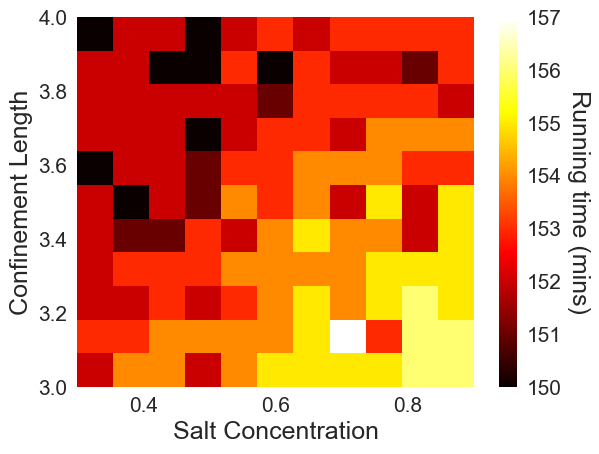
\includegraphics[width=0.3\textwidth]{../graphs/hmap.png}
%     \vspace*{\myfigspace}
%   \caption{Running times of the Nanoconfinement application with different sets of parameters have low variation.}
%   \label{fig:heatmap}
%   \vspace*{\myfigspace}
% \end{figure}

Large computational requirements of scientific simulations make them ideal for low-cost transient servers. 

The typical workflow associated with most scientific computing applications, often involves evaluating a computational model across a wide range of physical and computational parameters. 
For instance, constructing and calibrating a molecular dynamics application (such as Nanoconfinement~\cite{jcs2}), usually involves running a simulation with different physical parameters such as characteristic sizes and interaction potentials, as well as computational parameters such as simulation timesteps. 
Each of these parameters can take a wide range of values, resulting in a large number of combinations which must be evaluated by invoking the application multiple times (also known as a parameter sweep). 
Since each computational job explores a single combination of parameters, this results in executing a ``bag of jobs'', with each job in the bag running the same application, but with possibly different parameters.


The bag of jobs execution model is pervasive in scientific computing and applicable in many contexts.
In addition to exploratory parameter sweeps, bags of jobs also result from running the application a large number of times to account for the model or computational stochasticity, and can be used to obtain tighter confidence intervals. 
Increasingly, bags of jobs also arise in the emerging research that combines statistical machine learning (ML) techniques and scientific simulations~\cite{ml.atomic2017,melko2017,sam2017}. %,fu2017,long2015machine, ferguson2017machine,ward2018matminer,jcs2,fox2019learning}.
For instance, large bags of jobs are run to provide the necessary training and testing data for learning statistical models (such as neural networks) that are then used to improve the efficacy of the simulations~\cite{jcs2}.


Bags of jobs are analogous to, but distinct from the bag of \emph{tasks} design~\cite{bot-2003}, where applications are decomposed into independent processes to enable flexible task scheduling. 
In contrast, the bags of jobs abstraction is independent of the application design---a bag of jobs may consist of a synchronous MPI program that is not amenable to flexible scheduling. 


%The bag of jobs resulting from exploratory parameter sweeps are an integral component in the model discovery and validation process, and ar

%More formally, a bag of jobs is defined as a collection of : \{Application, $N$: Number of jobs, $m$: Minimum number of jobs to finish, $\pi$: Generator function for job parameters, $\mathcal{R}$: Computing resources per job\}

The bag of jobs execution model has multiple characteristics, that give rise to unique challenges and opportunities when deploying them on transient cloud servers. 
Since bags of jobs require a large amount of computing resources, deploying them on the cloud can result in high overall costs, thus requiring policies for minimizing the cost and overall running time. 
The similarity in execution characteristics of jobs (such as their running times and parallel speedup) allows for bag-wide optimizations (Figure~\ref{fig:heatmap}). 
%Second, there is no dependency between individual jobs in a bag, thus allowing increased flexibility in job scheduling.
And last, treating entire bags of jobs as an execution unit, instead of individual jobs, can allow us to use partial redundancy between jobs and reduce the fault-tolerance overhead to mitigate transient server preemptions. 



% We will modify our text to safeguard against R2's misunderstanding.
% statistical pattern recognition/machine guessing 
%%% Local Variables:
%%% mode: latex
%%% TeX-master: "paper"
%%% End:

%
\section{Background}

\subsection{Transient Computing}

%\subsection{Heterogeneity and Parallel Scientific Applications in the Cloud}

%No extra parallelism required
%RM heterogen

%
\subsection{Case Studies: Bags of Jobs in Scientific Computing Applications}

\begin{comment}
Describe the kind of computation. DONE

Scaling properties. Almost perfectly scalable with O(n) communication? UNCLEAR WHAT IS MEANT TO BE DONE HERE

This can be a like a case study of parallel scientific simulations.
Will help relate to parameters etc with more concrete examples. DONE

Bag of jobs.
Why multiple runs: parameter sweeps, search, or just multiple times to get confidence intervals and stable results in case of randomness. 
DONE I THINK
\end{comment}

For testing and evaluating the SciSpot framework, we consider three representative examples (case studies) from molecular dynamics (MD) and hydrodynamics simulations: 1) MD simulations of ions in nanoscale confinement created by material surfaces \cite{jjzo1,kadupitiya2017}, MD-based optimization dynamics of shape-changing deformable nanoparticles (NPs) \cite{jto1,jyto}, and hydrodynamics simulations of continuum material models using the Livermore Unstructured Lagrangian Explicit Shock Hydrodynamics (LULESH) code \cite{IPDPS13:LULESH,LULESH2:changes}. These examples are representative of typical scientific computing applications in the broad domain of physics, materials science, and chemical engineering; the first two applications (1 and 2) are based on codes and associated theoretical formulations developed by us \cite{jso1,jso2,solis2013generating,jjzo1,jto1,jyto}, and case study 3 is based on an open-source code developed at Lawrence Livermore National Laboratories \cite{IPDPS13:LULESH,LULESH:spec}. These three examples are implemented as parallel programs that use OpenMP and MPI parallel computing techniques.

The typical workflow associated with most scientific computing applications, including the aforementioned case studies, involves the implementation of the ``bags of jobs'' approach at many critical stages. In the initial stage, the construction and calibration of the appropriate model often involves testing for the needed attributes (e.g., characteristic sizes, interactions potentials) of the building blocks (model components) by sweeping over different combinations of physical as well as computing parameters (e.g., simulation timestep, thermostat variables) and eliminating the sets that lead to unphysical, unstable, or computationally intractable scenarios. During the model examination stage for the investigation of the accuracy and generalization of the model to describe the associated natural or synthetic processes, the dynamics of the model system is simulated over a wide range of model parameters. Accordingly, multiple sets of simulations (bags of jobs) are run to sweep over a broad region of the multidimensional parameter space and to isolate the domains where the model works best and where it yields a poorer representation of the real system. 

Often, the key objective of the scientific computing application is to isolate the model system parameters where interesting changes in the material structure or assembly behaviors (e.g., phase transitions) are observed. A similar bags of jobs approach is also  adopted in such applications with the search for these model parameters generally inspired by experimentally-informed observations and/or predictions yielding from approximate analytical theoretical formulations. For example, in the simulation of deformable nanoparticles implemented in the NP shape code, one is interested in isolating the set of NP and environmental parameters: NP bending modulus, NP stretching constant, NP charge, and salt concentration, that yields complex NP deformations/shapes (e.g., discs, rods, bowls). Similarly, in the ions in nanoconfinement application, a quantity of interest is the set of electrolyte system attributes (parameters): confinement length $h$, positive ion valency ($z_p$), negative ion valency ($z_n$), electrolyte concentration $c$, and ion diameter $d$, that yields the expected contact density or the experimentally-measured effective pressure between the confining nanomaterial surfaces. Finally, the bags of jobs approach is adopted during the completion process in the workflow where simulations are often launched in parallel to fill any gaps in the extracted trends or to obtain error bars on the predictions (e.g., ionic density profiles, energy distributions, NP shape transitions).

In addition to the conventional scientific computing (HPC) applications, an emerging area of research in a broad range of fields including materials science, biology, neuroscience, and physics where the bags of jobs approach is critical to the workflow is the integration of machine learning (ML) tools with these HPC applications  \citep{ml.atomic2017,melko2017,sam2017,fu2017,long2015machine, ferguson2017machine,ward2018matminer,jcs1,jcs2,fox2019learning}. ML methods have been developed and implemented to identify model attributes/parameters that yield desirable material configurations \citep{glotzer2017}, update configurations in simulations \citep{botu2015adaptive,fu2017}, predict and auto-tune optimal simulation control parameters \cite{jcs1}, predict critical features associated with simulation output \cite{jcs2}, infer assembly landscapes \citep{long2015machine,ferguson2017machine}, and classify phases of matter \citep{melko2017}. In many of these examples, ML models (e.g., artificial neural network, support vector machines) are trained on large data sets generated via simulations run over a broad range of parameter values. The bags of jobs process is invoked multiple times during the experimentation with many ML techniques using training and testing datasets to isolate the ML method(s) that yield the most accurate results for a given scientific computing application. For example, in Ref.~\cite{jcs2}, an ANN was trained to predict contact, peak, and mid-point ionic density using training and testing datasets comprising of $\approx4800$ and $\approx2000$ simulation runs respectively. Datasets were generated using HPC resources (Bigred2 computing cluster) based on the sweep of parameters $h \in (3.0, 4.0)$ nm,  $z_p \in 1,2,3$ (in units of electronic charge $|e|$); $z_n \in -1,-2$ $|e|$; $c \in (0.3,0.9)$ M, and $d \in (0.5,0.75)$ nm. We envision the SciSpot framework described here to complement and supplement conventional HPC supercomputer systems in enabling the construction of such ML layers (wrappers) \cite{jcs2,fox2019learning} around scientific computing applications. 

%%% Local Variables:
%%% mode: latex
%%% TeX-master: "paper"
%%% End:


%\section{Understanding and Modeling Transient Server Preemptions}
%\section{Modeling the Dynamics of Transient Server Preemptions}
%\section{Preemption Dynamics of Transient Cloud Servers}
\vspace*{\subsecspace}
\section{Constrained Preemptions of Google Preemptible VMs}
\label{sec:failmodel}

%Understanding the nature and dynamics of transient cloud servers such as their preemption frequency is a prerequisite to understand and improve the performance of applications.

%This is presumably in the background 
\eat{In order to understand and improve the performance of applications running on transient cloud servers, we must understand the nature and dynamics of their preemptions.
The preemption characteristics are governed by the supply of surplus resources, the demand for cloud resources, and the resource allocation policies enforced by the cloud operator.
Therefore, in this section, we present empirical and analytical models to help us understand the nature of preemptions. 
}

%To measure and improve the performance of applications running on transient cloud VMs, it is critical to understand the nature and dynamics of their preemptions.
%
In this section, we first present an empirical analysis of preemptions of Google Preemptible VMs, and then develop a new  probability model based on our observations. 
Finally, we discuss the unique aspects and general characteristics of constrained preemptions using reliability theory and statistical mechanics.


%and present  general observations about constrained preemptions using statistical mechanics. 

%The preemption characteristics are governed by the supply of surplus resources, the demand from applications, and resource allocation policies of the cloud operator.


%that describe these characteristics and enable an intuitive understanding of the nature of preemptions. 


% Transient cloud servers, by their very nature have limited availability and are frequently preempted.
% These preemptions are akin to fail-stop failures, and are often preceeded by a small advance warning (few seconds) to allow for graceful shutdowns.

% Since preemptions can impact the availability, performance, and cost of running applications, in this section, we examine their preemption characteristics.
% This modeling is important, because having a model of the availability can be useful in the context of predicting the running times of applications.
% Cloud providers offer a large number of servers of different configurations and types.
% Since transient server availability is fundamentally tied to supply and demand, the availability of servers of different types can be significantly different. 
% Thus, selecting the ``right'' server type is crucial for minimizing the overall costs. 



%\cite{alicloud-spot, packet-spot}

%\subsection{Empirical model of preemptions}
%\subsection{Empirical preemption behavior}
%\vspace*{\subsecspace}
\subsection{Empirical Study Of Preemptions}

% The preemptions of transient servers need not be related to their price.

\begin{figure}
  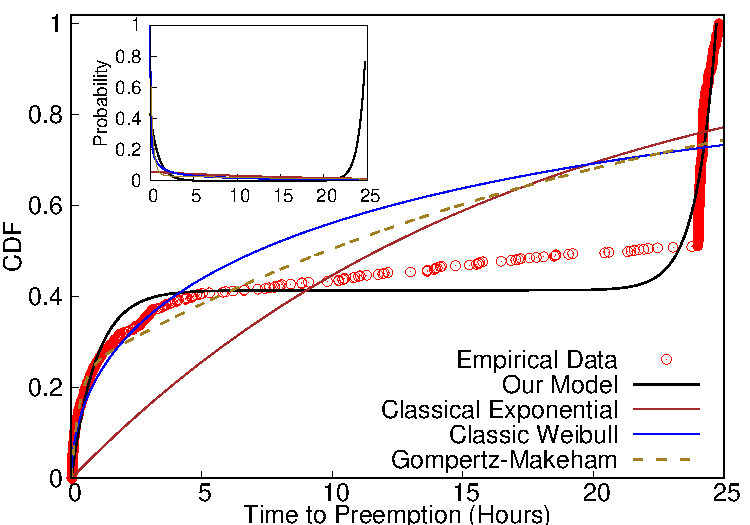
\includegraphics[width=0.47\textwidth]{../data/gnuplot-figures/sigmetrics-fig-cdf-prob-inset-time.pdf} 
  \caption{CDF of lifetimes of Google Preemptible VMs. Our proposed distribution for modeling the constrained preemption dynamics provides better fits to the empirical data compared to other failure distributions. Inset shows the probability density functions.}
  \label{fig:gcp1}
\end{figure}

To understand the nature of temporally constrained preemptions, we conducted the first empirical study of Google's Preemptible VMs, that have a fixed price and a maximum 24 hour lifetime.
Our empirical study is necessitated by the fact that the cloud operator (Google) does not disclose any other information about the preemption rates, and thus relatively little is known about the preemptions of these VMs, and as a result their performance.


We launched  1,516 Google Preemptible VMs of different types over a two month period (Feb--April 2019), and measured their time to preemption (i.e., their useful lifetime).\footnotemark
To ensure the generality of our empirical observations, VMs of different resource capacities were launched in a four geographical regions; during days and nights and all days of the week; and running different workloads. 
%
\footnotetext{We will release the complete preemption dataset for further analysis.} %Weaksauce 
%
A sample of over 100 such preemption events are shown in Figure~\ref{fig:gcp1}, which shows cumulative distribution function (CDF) of the VM lifetimes of the \texttt{n1-highcpu-16} VM in the \texttt{us-east1-b} zone. 
%enter the type of VM for which the data is shown
Note that the cloud operator (Google) caps the \emph{maximum} lifetime of the VM to 24 hours, and all the VMs are preempted before that limit. 

\begin{figure*}
  %\centering
  \subfloat[Preemption characteristics of different VM types. Larger VMs are more likely to be preempted.
  \label{fig:cdf-comparison}]
  {  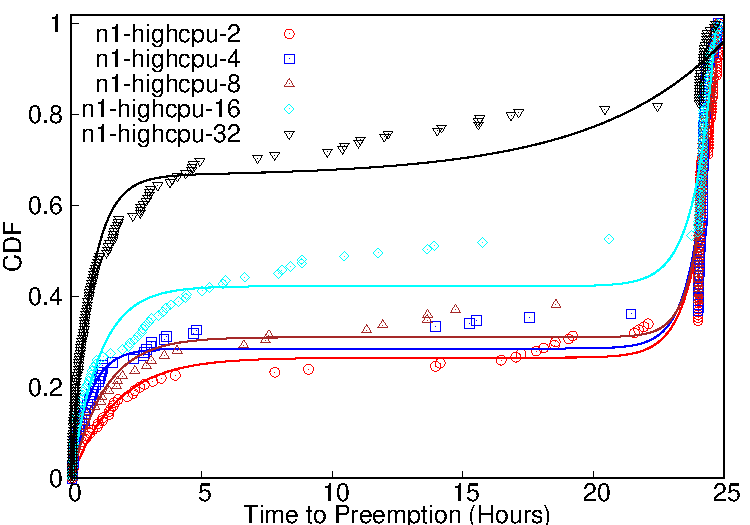
\includegraphics[width=0.3\textwidth]{../data/gnuplot-figures/sigmetrics-fig-vm-types.pdf} }
  \hfill
\subfloat[Variations due to time of day and workload. \label{fig:time-breakdown}]
{  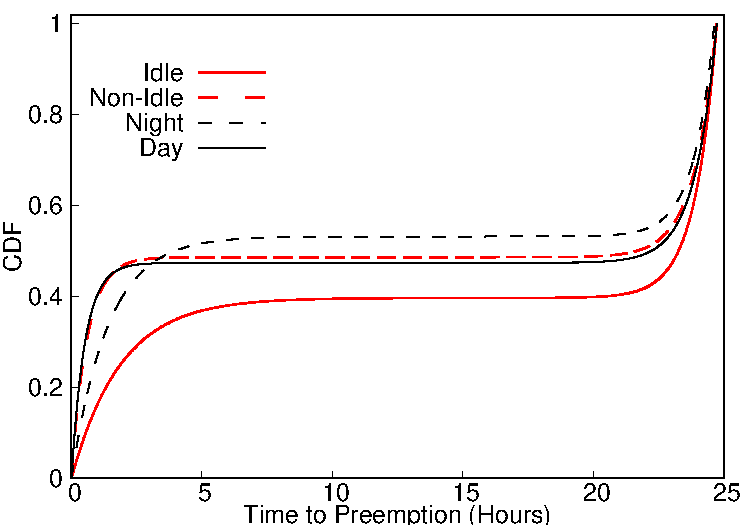
\includegraphics[width=0.3\textwidth]{../data/gnuplot-figures/sigmetrics-time-breakdown.pdf} }
\hfill
\subfloat[\textbf{n1-highcpu-16} in different regions. \label{fig:region-breakdown}]
{  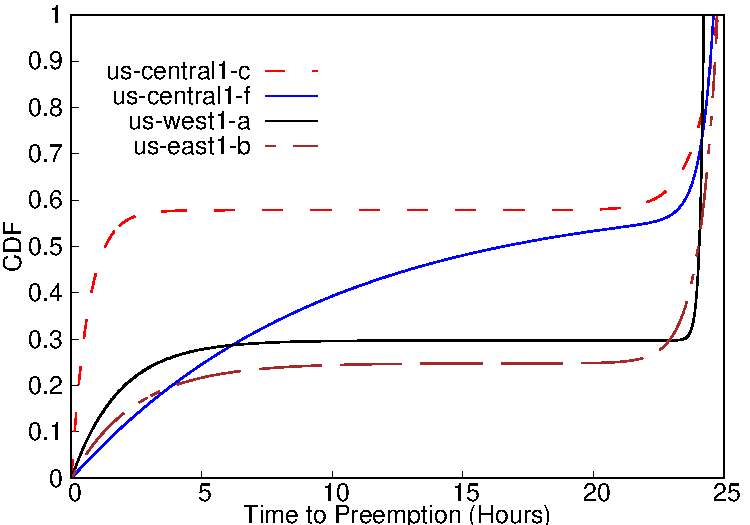
\includegraphics[width=0.3\textwidth]{../data/gnuplot-figures/sigmetrics-region-breakdown.pdf} }
\vspace*{-0.6cm}
\caption{Analysis of preemption characteristics by VM-type, region, time-of-day, and workload type.}
\label{fig:breakdown-all}
    \vspace*{\myfigspace}
\end{figure*}

\noindent \textbf{Observation 1:} \emph{The lifetimes of VMs are not uniformly distributed, but have three distinct phases.}

\noindent In the first (initial) phase, characterized by VM lifetime $t\in [0, 3]$ hours, we observe that many VMs are quickly preempted after they are launched, and thus have a steep rate of failure. The rate of failure (preemption rate) is the derivative of the CDF.
%; the rate of failure or preemptions can be obtained by taking the derivative of the CDF. 
In the second phase, VMs that survive past 3 hours enjoy a relatively low preemption rate over a relatively broad range of lifetime (characterized by the slowly rising CDF in Figure~\ref{fig:gcp1}).
The third and final phase exhibits a steep increase in the number of preemptions as the preemption deadline of 24 hours approaches.
The overall rate of preemptions is ``bathtub'' shaped as shown by the solid black line in the inset of Figure~\ref{fig:gcp1} (discussed in detail below).
%\it I think we should show the probability plot to exhibit the bath tub shape

%The preemption rate is ``bath tub'' shaped, with VMs that survive past 3 hours enjoying a relatively low preemption rate, and finally a steep increase in the number of preemptions as the preemption deadline (24 hours) approaches. 


\noindent \textbf{Observation 2:} \emph{The preemption behavior, imposed by the constraint of the 24 hour lifetime, is substantially different from conventional failure characteristics of hardware components and EC2 spot instances.}

\noindent In ``classical'' reliability analysis, the rate of failure  usually follows an exponential distribution $f(t) = \lambda e^{-\lambda t}$, where $\lambda=1/\text{MTTF}$.
Figure~\ref{fig:gcp1} shows the CDF ($=1-e^{-\lambda t}$) of the exponential distribution when fitted to the observed preemption data, by finding the distribution parameter $\lambda$ that minimizes the least squares error.
The classic exponential distribution is unable to model the observed preemption behavior because it assumes that the rate of preemptions is independent of the lifetime of the VMs, i.e., the preemptions are \emph{memoryless}.
%The primary reason is that the exponential distribution assumes that the \vj{the rate of preemptions is independent of the lifetime of the VMs} (preemptions are \emph{memoryless}), which does not hold true when there is a fixed upper bound on the lifetime, as is the case for Google Preemptible VMs. \vj{In other words, the conventional approach is insufficient to model constrained preemption dynamics.}
%We attribute this deficiency to the central assumption made in the underlying reliability theory principles that leads to the classical exponential distribution: the rate of preemptions is independent of the lifetime of the VMs, in other words, the preemptions are \emph{memoryless}.
This assumption breaks down when there is a fixed upper bound on the lifetime. %, as is the case for Google Preemptible VMs.%, and the conventional approach becomes insufficient to model this constrained preemption dynamics. 

\noindent \textbf{Observation 3:} \emph{The three preemption phases and associated bathtub shaped preemption probability are general, universal characteristics of Preemptible VMs.}

In general, the preemption dynamics of a VM are determined by the supply and demand of VMs of that \emph{particular} type.
Thus, our empirical study looked at preemptions of VMs of different sizes, in different geographical zones, at different times of the day, and running different workloads (Figure~\ref{fig:breakdown-all}).
In all cases, we find that there are three distinct phases associated with the preemption dynamics giving rise to the bathtub shaped preemption probability. 
We argue that this is not a coincidence, but may be a result of practical and fundamental outcomes of cluster management policies. 

While the actual specific preemption policy is up to the cloud operator, we will show that the bathtub behavior has benefits for applications. 
%The bathtub behavior results in a high rate of failure initially. 
For applications that do not incorporate explicit fault-tolerance (such as checkpointing), early preemptions result in less wasted work than if the preemptions were uniformly distributed over the 24 hour interval.
Furthermore, the low rate of preemptions in the middle periods allows jobs that are smaller than 24 hours to finish execution with only a low probability of failure, once they survive the initial preemption phase. 
We evaluate the performance of applications with bathtub shaped preemptions in Section~\ref{sec:eval}. 
%
In addition to being beneficial to applications, we also conjecture that the bathtub behavior may be  a \emph{fundamental} and general characteristic of constrained preemptions, which we show later in Section~\ref{subsec:stat-mech}. 
%system where events are randomly distributed in a finite interval later in Section~\ref{subsec:stat-mech}. 
%
%Intriguingly, we can analyze such temporally constrained preemptions through a statistical mechanics framework, and we elaborate on this connection later in Section~\ref{subsec:statmech}.


\noindent \textbf{Observation 4:}\emph{ Larger VMs have a higher rate of preemptions.}

Figure~\ref{fig:cdf-comparison} shows the preemption data from five different types of VMs in the Google Cloud \texttt{n1-highcpu-\{2,4,8,16,32\}}, where the number indicates the number of CPUs.
All VMs are running in the \texttt{us-central1-c} zone. 
We see that the larger VMs (16 and 32 CPUs) have a higher probability of preemptions compared to the smaller VMs.
While this could be simply due to higher demand for larger VMs, it can also be explained from a cluster management perspective. 
Larger VMs require more computational resources (such as CPU and memory), and when the supply of resources is low, the cloud operator can quickly reclaim a large amount of resources by preempting larger VMs.
This observed behavior aligns with the guidelines for using preemptible VMs that suggests the use of smaller VMs when possible~\cite{preemptible-documentation}. 

\noindent \textbf{Observation 5:} \emph{Preemptions exhibit diurnal variations, and are also affected by the workload inside the VM.}

From Figure~\ref{fig:time-breakdown}, we can see that VMs have a slightly longer lifetime during the night (8 PM to 8 AM) than during the day.
This is expected because fundamentally, the preemption rates are higher during periods of higer demand. 
%
We also notice that completely idle VMs have longer lifetimes than VMs running some workload.
Presumably, this could be a result of the lower resource utilization of idle VMs being more amenable to resource overcommitment, and result in lower preemptions. 

\begin{figure}
  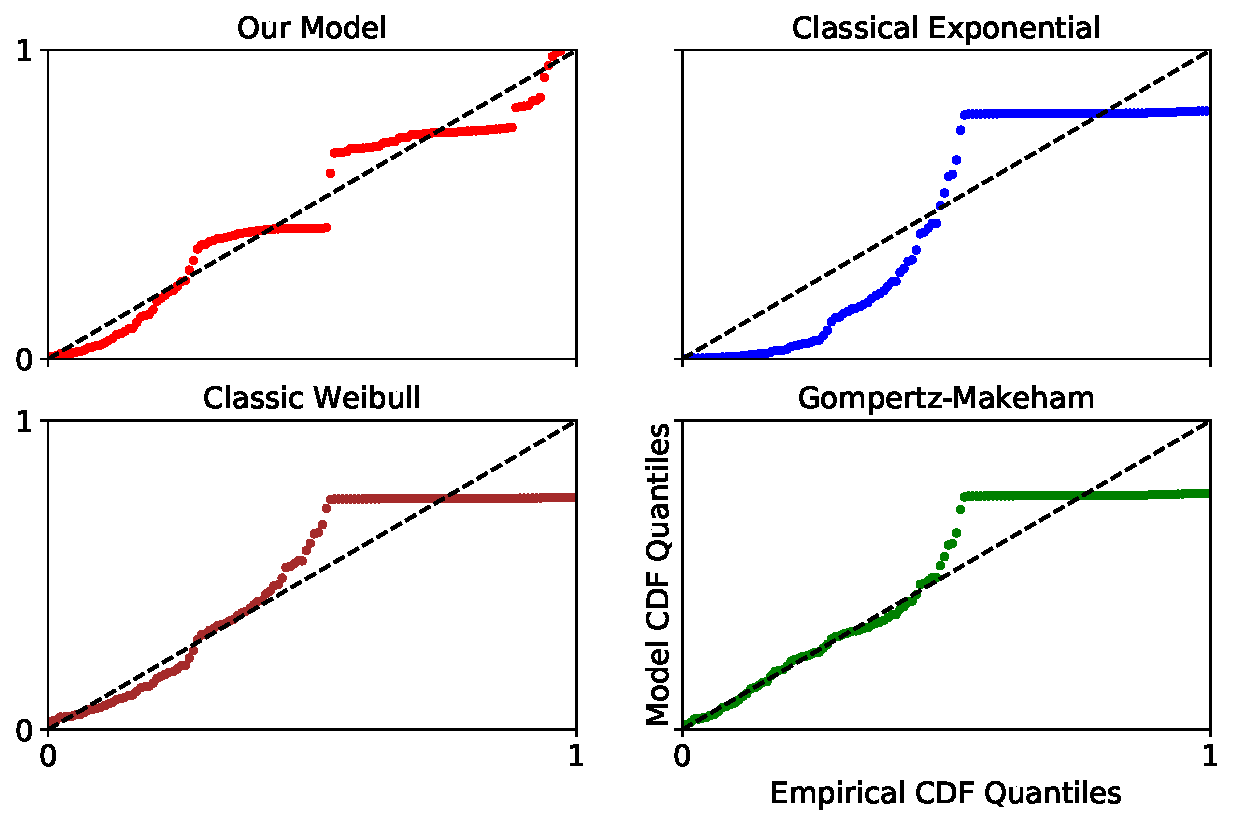
\includegraphics[width=0.4\textwidth]{../graphs/QQ.pdf}
    \vspace*{-5pt}
  \caption{QQ plot of different preemption models. Existing models are unable to capture all the preemption phases.}
  \label{fig:QQ}
  \vspace*{-5pt}
\end{figure}

%being more amenable to resource overcommitment, and therefore don

%%%%%%%%%%%%%%%%%%%%%%%%%%%%%%%%%%%%%%%%%%%%%%%%%%%%%%%%%%%%%%%%%%%%%%

\vspace*{\subsecspace}
\subsection{Failure Probability Model}
\label{subsec:analytical-model}

%Based on our empirical analysis of preemptions,  
We now develop an analytical probability model for finding a preemption at time $t$ (preemption dynamics) that is faithful to the empirically observed data and provides a basis for developing running-time and cost-minimizing optimizations. %
Modeling preemptions constrained by a finite deadline raises many challenges for existing preemption models that have been used for other transient servers such as EC2 spot instances. 
We first discuss why existing approaches to preemption modeling are not adequate, and then present our closed-form probability model and associated reliability theory connections. 

%How to avoid sounding like the background section?

\subsubsection{Inadequacy of existing failure distributions}

Spot instance preemptions have been modeled using exponential distribution~\cite{bid-cloud, hotcloud-not-bid, flint}, which is the default in most reliability theory applications. 
However, the strict 24 hour constraint and the distinct preemption phases are not compatible with the memoryless properties of the exponential distribution. 
%
To describe failures (preemptions) that are not memoryless (i.e., increasing or decreasing failure rate over time), the classic Weibull distribution with CDF $F(t)=1-e^{-(\lambda t)^k}$ is often employed. However, the Weibull distribution is also unable to fit the empirical data (Figure~\ref{fig:gcp1}) and especially unable to model the sharp increase in preemptions near the 24 hour deadline. 

For constrained preemptions, the increase in failure rate as modeled by the Weibull distribution is not high enough.
Other distributions, such as Gompertz-Makeham, have also been used for modeling bathtub behavior, especially  for actuarial use-cases~\cite{missov2013gompertz}. 
The key idea is to incorporate an exponential aging process, which is used to model human mortality.
The CDF of the Gompertz-Makeham distribution is given by $F(t) = 1 - \exp\left(-\lambda t - \dfrac{\alpha}{\beta}(e^{\beta t} - 1) \right)$
  and is fitted to the data in Figure~\ref{fig:gcp1}, and is also unable to provide a good model for the observed preemption data. 

%Specifically, it is unable to model the bathtub preemption rate and the different preemption phases, and 


%We also analyze other distributions used for modeling bathtub failures from reliability and actuarial theory in Figure \textbf{XXX}.


The non-trivial bathtub-shaped failure rate of Google preemptible VMs (Figure~\ref{fig:gcp1}) requires models that capture the sudden onset of the rise in preemptions near the deadline.
From an application and transiency policy perspective, the preemption model must provide insights about the phase transitions, so that the application can adapt to the sharp differences in preemption rates.
%
For example, the preemption model should be able to warn applications about impending deadline, which existing failure distributions cannot account for. 
% which imposes a dynamics that is more akin to a constrained dynamics problem as opposed to dynamics characterized with a gradually rising failure rate.
Thus, not only is it important to minimize the total distribution fitting error, it is also important to capture the changes in phase.
However, as we can see from Figure~\ref{fig:QQ}, existing distributions are unable to capture the effects of the deadline and the phases of the preemptions, and a new modeling approach is needed, which we develop next.  

\subsubsection{Our  model}
\label{subsec:preemption-model}


%This is especially important from a policy design perspective, as the ``phase changes'' in preemption behavior can greatly affect the failure probability and performance of applications.
%Our new model, informed by the cumulative distribution of lifetimes that has multiple distinct temporal phases, addresses this need.

Our failure probability model seeks to address the drawbacks of existing reliability theory models for modeling constrained preemptions. 
The presence of three distinct phases exhibiting non-differentiable transition points (sudden changes in CDF near the deadline, for example) suggests that for accurate results, models that treat the probability as a step function (CDF as a piecewise-continuous function) should be employed. However, this limits the range of model applicability and general interpretability of the underlying preemption behavior. Our goal is to provide a broadly applicable, continuously differentiable, and informative model built on reasonable assumptions.  

We begin by making a key assumption: the preemption behavior arises from the presence of \emph{two} distinct failure processes.
%that give rise to a new probability distribution characterizing the preemptions and the observed CDF, and ensure the dependence of the rate of failure on the VM lifetime. 
The first process dominates over the initial temporal phase and yields the classic exponential distribution that captures the high rate of early preemptions.
The second process dominates over the final phase near the 24 hour maximum VM lifetime and is assumed to be characterized by an exponential term that captures the sharp rise in preemptions that results from this constrained lifetime. 
%Generally, these two processes jointly determine the dynamics of preemptions during the middle phase where a relatively constant or a slowly rising number of preemptions with time is observed.
%; in practice, based on the fits to the empirical data, we observe the first process to dominate over the second during this phase as well. 

%The first two phases are reasonably captured by the classic exponential distribution. In order to model the overall observed empirical CDF, we add another term that captures the failure process near the 24 hour maximum VM lifetime,  and construct a \emph{new} probability distribution. 
%
%we develop a \emph{new} probability distribution that is composed by blending two failure processes that act on different temporal phases over the 24 hour maximum lifetime of the VMs. 
%
%We write the general form of our blended preemption CDF as follows:

Based on these observations, we propose the following general form for the CDF:

\vspace*{\subsecspace}
\begin{equation}
  \label{eq:blend1}
  \boxed{
  \mathscr{F}\left(t\right) = A\left(1-e^{-\frac{t}{\tau_1}} + e^{\frac{t-b}{\tau_2}}\right)}
  \end{equation}
\noindent where $t$ is the time to preemption, $1/\tau_1$ is the rate of preemptions in the initial phase, $1/\tau_2$ is the rate of preemptions in the final phase, $b$ denotes the time that characterizes ``activation'' of the final phase where preemptions occur at a very high rate, and $A$ is a scaling constant. 
%
The model is fit to data for $0 < t < L$, where $L \approx 24$ hours represents the temporal interval (deadline).
Combination of the 4 fit parameters ($\tau_1, \tau_2, b$, and $A$) are chosen to ensure that boundary condition $\mathscr{F}(0) \approx 0$ is satisfied.
%and $\mathscr{F}(L) \approx 1$. 
%%When not used as a fit parameter, $A$ is chosen as $A = 1/(1-e^{-\frac{L}{\tau_1}} + e^{\frac{L-b}{\tau_2}})$ to ensure $F(L) = 1$, yielding results similar to the 4 parameter fit. 
In practice, typical fit values yield $b \approx 24$ hours, $\tau_1 \in [0.5, 0.8] $, $\tau_2 \approx 1$ hour, and $A \approx 0.7$.



%\vikram{check, and provide typical fit values for all these parameters as well as their range extremes. ideally, you want to fit with A set to the above expression to avoid any $\mathscr{F}(t)$ or $p(t)$ > 1 scenarios. turns out that having A is important in reliability analysis -- check next column}


%of  0 $\approx 0$ premptions.
%used to scale the CDF to ensure that the initial conditions ($F(0)=0$) are met.

For most of its life, a VM sees failures according to the classic exponential distribution with a rate of failure equal to $1/\tau_1$ -- this behavior is captured by the $1-e^{-t/\tau_1}$ term in Equation~\ref{eq:blend1}. 
%However, this does not capture the finite lifetime of the VM imposed by the cloud operator.
As VMs get closer to their maximum lifetime imposed by the cloud operator, they are reclaimed (i.e., preempted) at a high rate $1/\tau_2$, which is captured by the second exponential term, $e^{(t-b)/\tau_2}$ of Equation~\ref{eq:blend1}. 
Shifting the argument ($t$) of this term by $b$ ensures that the exponential reclamation is only applicable near the end of the VM's maximum lifetime and does not dominate over the entire temporal range. 
%As noted before, $1/\tau_2$ is the rate of this reclamation. 

The analytical model and the associated  distribution function $\mathscr{F}$ introduced above provides a much better fit to the empirical data (Figure~\ref{fig:gcp1}) and captures the different phases of the preemption dynamics through parameters $\tau_1, \tau_2, b$, and $A$. These parameters can be obtained for a given empirical CDF using least squares function fitting methods (we use scipy's \texttt{optimize.curve\_fit} with the dogbox technique~\cite{scipy-fit}). The failure or preemption rate can be derived from this CDF as:
\begin{equation}
  \label{eq:failrate}
    \vspace*{\eqnspace}
f(t) = \dfrac{d \mathscr{F}(t)} {dt} = A \left(\dfrac{1}{\tau_1}e^{-t/\tau_1} + \dfrac{1}{\tau_2}e^{\frac{t-b}{\tau_2}}\right).
\end{equation}
$p(t)$ vs. $t$ yields a bathtub type failure rate function for the associated fit parameters (inset of Figure~\ref{fig:gcp1}).
%In the next section, we use this analytical model for optimizing cloud resource selection to run scientific computing applications at low cost and shorter running (turnaround) times.


In the absence of any prior work on constrained preemption dynamics, our aim is to provide an interpretable model with a minimal number of parameters, that provides a sufficiently accurate characterization of observed preemptions data. 
%As is evident from Figure~\ref{fig:gcp1}, our model shows deviations from the data near the halfway point within the 24 hour lifetime. 
Further generalization of this model to include more failure processes would introduce more parameters and reduce the generalization power. 
%Exploring other approaches of modeling bathtub-type failure rates (e.g., exponential Weibull distributions) \cite{mudholkar1993exponentiated,crevecoeur1993model} is part of our future work. 


\subsubsection{Reliability Analysis}
\label{subsec:reliability}

We now analyze and place our model in a reliability theory framework. 
%

\noindent \textbf{Expected Lifetime:} Our analytical model also helps crystallize the differences in VM preemption dynamics, by allowing us to easily calculate their expected lifetime. 
More formally, we define the expected lifetime of a VM as: 
\begin{equation}
  \label{eq:expected-lifetime}
E[L] =  \int_{0}^{24} t {f}(t)~dt =  -A(t+\tau_1)e^{-t/\tau_1} + A(t-\tau_2) e^{\frac{t-b}{\tau_2}} \biggr\rvert_{0}^{24}
\end{equation}
where $f(t)$ is the rate of preemptions of the VM (Equation~\ref{eq:failrate}).
%= \dfrac{d \mathscr{F}(t)} {dt} = A \left(\dfrac{1}{\tau_1}e^{-t/\tau_1} + \dfrac{t-b}{\tau_2}e^{\frac{t-b}{\tau_2}}\right) $ 
%
%Since preemptions require restarting a job and increase the job completion time, it may be more prudent to select transient VMs with higher expected lifetimes.

This expected lifetime can be used in lieu of MTTF, for policies and applications that require a ``coarse-grained'' comparison of the preemption rates of servers of different types, which has been used for cost-minimizing server selection~\cite{flint}. 

%We use the analytically derived expected lifetimes of VMs of different types in \sysname when selecting the ``best'' VM type for a given bag of jobs. This server selection is a key part of \sysname design. 

\noindent \textbf{Hazard Rate:}
The hazard rate $\lambda(t)$ governs the dynamics of the failure (or survival) processes. It is generally defined as $\lambda(t) = \frac{g(t)}{S(t)}$, often expressed via the following differential equation (rate law):
\begin{equation}\label{eq:hazard}
\frac{dS(t)}{dt} = -\lambda(t) S(t)
\end{equation}
%$\lambda(t) = \frac{f(t)}{S(t)}$ \vikram{this was inverted, I fixed. double check please}, 
where $S(t) = 1 - F(t)$ is the survival function associated with a CDF $F(t)$, and $g(t)=dF(t)/dt$ is the failure probability function (rate) at time $t$. The survival function indicates the amount of VMs that have survived at time $t$.
The hazard rate can also be directly expressed in terms of the CDF as follows: $1-F(t) = \exp{\int_0^t{-\lambda(x) ~dx}}$. 
The exponential distribution has a constant hazard rate $\lambda$.
The Gompertz-Makeham distribution has an increasing failure rate to account for the increase in mortality, and its hazard rate is accordingly non-uniform and given by $\lambda(t) = \lambda + \alpha e^{\beta t}$.

Since we model multiple failure rates and deadline-driven preemptions, our hazard rate is expected to increase with time. Defining the survival function for our model: $S = 1 - \mathscr{F}$, and using Eq.~\ref{eq:hazard} yields the hazard rate associated with our model: 
%$\lambda(t) = \dfrac{- r_1 e^{- r_1 t} - r_2 e^{r_2 (t - b)}}{e^{- r_1 t} - e^{r_2 (t - b)}}$. 
% missing minus sign in the above equation
\noindent 
\begin{equation}
  \label{eq:hmodel}
  \lambda %= r_2 + \bar{r} \left( \dfrac{1}{1 - e^{- r_2 b} e^{\bar{r} t}}\right)
  %= \dfrac{r_1 + r_2 e^{- r_2 b} e^{\bar{r} t}}{1 - e^{- r_2 b} e^{\bar{r} t}}.  
  = \dfrac{r_1 e^{- r_1 t} + r_2 e^{r_2 (t - b)}}{1/A - 1 + e^{- r_1 t} - e^{r_2 (t - b)}}
\end{equation}
where we have introduced $r_1 = 1/\tau_1$, $r_2 = 1/\tau_2$ to denote the rates of preemptions associated with initial and final phases respectively.

%\vikram{without the A term, hazard rate becomes negative for the older expression you had when $t > b r2 / (r1+r2)$. that is for t roughly greater than b/2, which is for more than 12 hours. hazard rate can never be negative.}
%Here we have introduced the sum of the two failure rate constants, $\bar{r} = r_1 + r_2$, to simplify the expression. \vikram{check}

%Employing the value for $A$ resulting from ensuring (via fit or by force) that our CDF goes to 1 at $t = L$ (where $L$ is 24 hours), we find

% \begin{equation}
%   \label{eq:hmodel2}
%   \lambda %= r_2 + \bar{r} \left( \dfrac{1}{1 - e^{- r_2 b} e^{\bar{r} t}}\right)
%   %= \dfrac{r_1 + r_2 e^{- r_2 b} e^{\bar{r} t}}{1 - e^{- r_2 b} e^{\bar{r} t}}.  
%   = \dfrac{r_1 e^{- r_1 t} + r_2 e^{r_2 (t - b)}}{e^{r_2 (L - b)}  - e^{- r_1 L} + e^{- r_1 t} - e^{r_2 (t - b)} }
% \end{equation}

Recall that the sharp increase in preemption rate only happens close to the deadline, which means that $b \lesssim L$. Thus, when $0 < t \ll b$, we get $\lambda(t) \approx r_1$, mimicking the hazard rate for the classic exponential distribution.
As $t$ approaches and exceeds $b$ (i.e., $b\lesssim t < L$), the increase in the hazard rate due to the second failure process kicks in, accounting for the deadline-driven rise in preemptions. Note that our hazard rate satisfies $\lambda(t) \ge 0$ for $0<t<L$.

% For ease of exposition, we can write this as:

% \begin{equation}
%  \label{eq:hmodelsimple}
% \lambda =  \dfrac{r_1 + \gamma_1 e^{\delta (t-b)}}{1 - \gamma_2 e^{\delta (t-b)}}
% \end{equation}
% 
% We note that the numerator is  similar to the hazard rate associated with Gompertz-Makeham distribution.
% The key difference is the $1-\gamma_2 e^{t-b}$ factor in the denominator. 
% Recall that the sharp increase in preemption rate only happens close to the deadline, which means that $b \leq 24$. Thus, when $t < b$, we get a conventional $\lambda = r_1$, or the classic exponential distribution.
% As $t$ approaches and exceeds $b$, the increase in failure rate kicks in, accounting for the deadline-driven rise in preemptions. 



% We emphasize that our motivation is to develop an interpretable \emph{minimal} model that provides a sufficiently accurate description of the observed constrained preemption dynamics of Google VMs with a minimal number of meaningful parameters. 
% As is evident from Figure~\ref{fig:gcp1}, $\mathscr{F}$ shows deviations from the data near the halfway point within the 24 hour lifetime.
% Further generalization of this model to include more failure processes, which would introduce more parameters, or exploring other approaches of modeling bathtub-type failure rates (e.g., exponential Weibull distributions) \cite{mudholkar1993exponentiated,crevecoeur1993model} may yield alternate model descriptions that capture the data with higher accuracy.


%PXXX part of future work? 

%characterized by failure rates and activation times (like $b$). 
%and reduce the predictive power and simplicity of the model. 
%We also note that approaches (e.g., exponential Weibull distributions) to model bathtub-type failure rates have been proposed in the literature  \cite{mudholkar1993exponentiated,crevecoeur1993model}.
%These methods did not perform better than our model resulting in parameter variables and values that were relatively difficult to interpret; this could likely be due to the unique constraint-driven failures in preemption dynamics as opposed to aging-related increasing failure rate considered in previous work. 

\subsection{Insights on the bathtub shape distribution}
\label{subsec:stat-mech}

For constrained preemptions, one might expect to see uniformly distributed preemptions with a probability $1/L$ over $[0, L]$. 
However, as our empirical analysis shows, the preemption distribution is baththub shaped.
Interestingly, we can show using exact analytical arguments that non-uniform, baththub distributions are in fact a \emph{general} characteristic of systems with constrained preemptions, modulo some assumptions. 

\begin{lemma}\label{lemma:1}
  Consider $N$ randomly distributed preemptions over an interval $[0, L]$.
  Assume that each preemption takes $w > 0$ time-units to perform, and preemptions cannot overlap, i.e, they occur in a mutually exclusive manner.
  Then, there exists $\epsilon > 0$ such that  $P(L-\epsilon) > \frac{1}{L}$, where 
 $P(t)$ is the probability of finding a preemption at time $t$. 
\end{lemma}


\begin{proof}
We first make some preliminary remarks and introduce concepts necessary to complete the proof. 

Firstly, mutual exclusion of preemptions implies that there is a finite non-zero waiting time $w>0$ between preemptions. 
For $N$ preemptions to occur within $L$ interval, evidently, we must have $Nw < L$. Also, while $w >0$, the time to perform the preemption is generally expected to be much smaller than the total time interval $L$.
$N$ preemptions occupy a ``temporal volume'' of $Nw$ (volume here represents the one-dimensional volume). We assume that while a preemption may start at $t=0$, the last preemption must finish by $t = L$. Thus, the amount of free or excluded ``temporal volume'' available within the constrained system is $L_e = L - w - (N-1)w = L - Nw$.
The idea of excluded volume is central in physics and materials engineering where it underpins the origin of entropic or steric forces in material systems \cite{krauth2006statistical,jing2015ionic}. 

Secondly, we note that the system of $N$ preemptions within a constrained deadline of interval $L$ maps \emph{exactly} to a well known and analytically solvable system in classical statistical mechanics, the Tonks gas model \cite{tonks}, where one considers a system of $N$ hard-spheres of diameter $w$ to move along a line segment of length $L$. The structural quantities associated with this system including the probability of finding a sphere at position $x$ within the interval $L$ are computed by evaluating the partition function of the system, which essentially measures the number of valid system configurations \cite{krauth2006statistical}. Employing this mapping and the associated statistical mechanics tools, the original model of non-overlapping (interacting) preemptions can be mapped to a system of $N$ overlapping (non-interacting) preemptions, each allowed to access an excluded volume of $L_e$, and the number of valid configurations is given by the partition function $Z_N = L_e^N$. For the case of $N$ preemptions, we have $Z_N = (L- Nw)^N$.

We are interested in calculating the probability that a preemption starts at time $t=L-w$, i.e., $P(L-w)$. Given that the time to perform the preemption $w$ is generally expected to be much smaller than the total time interval $L$, $P(L-w)$ is the probability of finding a preemption near the deadline. The assumption of mutually exclusive preemptions implies that no other preemption can be found for $t > L - w$, that is, $P(t> L-w) = 0$. Hence, the remaining $N-1$ preemptions must occur such that the last of those finish by $t=L-w$ (the preemption at time $L-w$ essentially sets an effective deadline for the other $N-1$ preemptions). The number of ways this can happen is given by the partition function $Z_{N-1} = L_e^{N-1}= (L-2w - (N-2)w)^{N-1} = (L - Nw)^{N-1}$, where $L_e = L - Nw$ is the corresponding excluded temporal volume accessible to each of the $N-1$ preemption. It is interesting to note that the excluded volume in this case is the same as that of the original $N$ preemption system: this fortuitous result arises because the reduction in available volume to place the preemptions is commensurate with the need to place $N-1$ preemptions instead of $N$.

The probability $P(L-w)$ is obtained as the ratio of the valid configurations given by the two partition functions computed above.
That is, 
$P(L-w) = Z_{N-1}/ {Z_N} = \frac{1}{L - Nw} > \frac{1}{L}$ , since $N \geq 1$ and $w>0$. Choosing $\epsilon = w > 0$ completes the proof.


%We begin by counting the total number of configurations available to place $N$ preemptions in the constrained temporal ``volume'' $L$. 
%The number of configurations one preemption can generate is proportional to the excluded volume available, i.e., $L-Nw$.
%For $N$ preemptions, the number of configurations grows exponentially and is proportional to the volume of the $N$-dimensional hypercube: $Z = (L-Nw)^N$. 
%This computation of the number of valid system configurations is in fact the partition function of the system in statistical mechanics~\cite{krauth2006statistical}. 

%Given the condition of mutually exclusive preemptions, we note that if we assume that there is a preemption at $t=L-w$, then $P(t> L-w) = 0$.
%For this case, the available, valid, non-overlapping configurations are proportional to the temporal volume accessible in the $N-1$ dimensional hypercube to $N-1$ preemptions: $Z_{1} = (L-w-(N-1)w)^{N-1} = (L-Nw)^{N-1}$. 

%The probability of finding 1 preemption near the deadline at $t=L-\epsilon$ when $\epsilon \in [w/2, w)$ is given as the ratio of the two computed volumes.
%That is, $P(L-\epsilon) = \frac{Z_1}{Z} = \frac{1}{(L - N\epsilon)} > \frac{1}{L}$ , since $N \geq 1$ and $\epsilon>0$. 
\end{proof}

By symmetry arguments, the above lemma is in fact valid for both the end points of the interval, i.e., $P(\epsilon) > \frac{1}{L}$.
Thus, the probability of preemption is higher near the end points (deadline) than the average preemption probability of $1/L$, and we get a bathtub shaped distribution.
Thus, the bathtub distribution can be considered to be a general artifact of constrained preemptions. Of course, the empirical preemption distribution is determined by the cloud platform's policies and supply and demand, and we elaborate more about the generality of our model and observation in Section~\ref{sec:discussion}. 

% How ?
%Crucial to our The assumption of preemption events

For the above proof, we assumed that each preemption event occurs over a timespan of $w$, which is determined by the preemption warning that the cloud platform provides (which is 30 seconds for Google Preemptible VMs and 120 seconds for Amazon EC2 spot instances). 
Preempting a VM and reclaiming its resources involves manipulating the cluster-management state, and mutually exclusive preemptions may be convenient for cluster management, since serializing VM preemptions makes accounting and other cluster operations easier.
From an application standpoint, non-overlapping preemptions are also beneficial, since handling multiple concurrent preemptions is significantly more challenging~\cite{exosphere}. 





\begin{comment}
\subsection{Elsewhere: Role of Cloud Providers: Analogy to Constrained Physical Systems}

The bathtub-shaped distribution of the preemption probability is essential to capture the empirical data with higher accuracy compared to other models. We want to probe the following question now: how much of this unique shape is enforced by the cloud provider, and how much is dictated by assuming that (akin to other cloud providers such as EC2), preemptions of Google Preemptible VMs are placed along the timeline of 24 hours with uniform probability? We make the question more precise and inject a relatively harmless assumption: if the cloud provider decides to ``place'' $N$ preemptions within the temporal boundary of interval $L$ with flat probability distribution ($\mathscr{P}(e_1, e_2, \ldots e_N)$ = 1 whenever legal) such that the preemptions are mutually exclusive (that is there is a finite non-zero waiting time between preemptions), what is the probability of finding a preemption at time $t$? Naively, deducing from $\mathscr{P}$, one may expect $p(t)$ to be 1 for $t\in L$, or a constant (flat) distribution. However, intruigingly, this is not true. Thus, as we discuss in more detail below, the cloud provider may have the simplest of preemption policies implemented at their end, and yet give rise to the relatively complex and non-trivial probability to preemption. 

To understand the above assertions with a simple example that sheds further insights into the origins of the bathtub-shaped distribution, we discuss analogous questions in the context of general physical systems of constrained (confined) particles.
These systems are generally analyzed using the theoretical framework of statistical mechanics often complemented with associated particle dynamics simulations. We choose an exactly solvable and simple system of hard (non-overlapping) particles (or beads) confined to move in one dimension within a finite spatial interval to draw interesting connections. 

A simple mapping from the system of temporally-constrained preemptions in the cloud to the system of spatially-constrained particles within one-dimensional confinement can be established by assuming that the cluster management policy requires mutually exclusive preemptions.
This assumption helps cluster management by serializing VM preemptions and making cluster operations easier, and it reduces the challenges associated with reacting to simultaneous preemptions. 
The preemption events become hard particles that cannot overlap. The preemption probability distribution gets mapped to the density of $N$ particles, each modeled as a one-dimensional ``sphere'' of width $\sigma$, confined in a 1-dimensional interval (line segment) of length $L$. $L$ can be considered as corresponding to the deadline interval of 24 hours. $\sigma$ is equivalent to the length of the critical section, which is related to the preemption warning (30 seconds for Google PVMs). 

The particles are placed, one after another, at random positions. Configurations where any overlap is generated are not included. Thus particles will be placed with a flat probability distribution.
The question we are trying to simulate with this set up is the familiar one noted above: what is the probability $p(x)$ of finding a preemption at time $x$?

This problem can be solved by first defining a partition function for the system. And doing some neat math.

Present the solution

This distribution is \emph{not} uniform over the interval, but is higher towards the ends of the interval---analogous to the bath-tub shaped nature of preemptions! 

Discuss more.

We thus draw a few critical observations.
An immediate inclincation may be to attribute the observed non-trivial bathtub-shaped preemption probability function to a uniquely designed and structured operational policy of the cloud provider. However, the above analysis shows that even with the vanilla operational policy of placing preemptions with a uniform probability distribution, the finite excluded temporal volume of preemptions in conjunction with the relatively short deadline (which together imply a high average preemption rate) enforce a bathtub-shape-like distribution for finding a preemption at time $t$. Clearly, this does not provide all the subtle features observed in the preemption data as well as the failure model. But even there, it enables to gauge the extent to which the provider has changed the policy on top of the simplest possible implementation.

The analytical framework suggests that the bath-tub shape of the probability distribution is the key characteristic of constrained preemptions.
Therefore, our approach will remain relevant in the face of future changes in preemption characteristics due to changes in cloud usage and operational policies.

\end{comment}

%These systems underlie a variety of phenomena in chemical and materials engineering applications such as ions confined in nanochannels \cite{jing,solis}. 

%In addition to empirically-informed reliability models for preemptions, we also seek to understand \emph{why} their distribution is bathtub shaped in order to provide a mechanistic understanding of preemptions and enhance the model interpretability and generalizability. 
%Our key insight is that the problem of analyzing constrained preemptions can be ``mapped'' to an equivalent problem in statistical mechanics of a physical system, and we can use the theoretical and analytical framework of statistical mechanics to develop a broader understanding of preemptions. 
%This connection to statistical mechanics is given below. 
%To this end, we propose to ``map'' the problem of constrained preemptions to an equivalent problem of constrained many particle physical systems that can be analyzed employing the general theoretical framework of statistical mechanics.

%A simple mapping can be established by assuming that the cluster management policy requires mutually exclusive preemptions.
%This assumption helps cluster management by serializing VM preemptions and making cluster operations easier, and it reduces the challenges associated with reacting to simultaneous preemptions. The preemption events become hard particles that cannot overlap. The probability distribution of $N$ constrained preemption events gets mapped to the density of $N$ randomly distributed particles confined in a 1-dimensional interval of length $L$ (analogous to 24 hours). 
%The particle size is equivalent to the length of the critical section, which is related to the preemption warning (30 seconds for Google PVMs).
%Finding the distribution of non-overlapping (i.e., hard) particles is a central problem in statistical mechanics [5].
%Interestingly, the distribution of particles in a confined interval can be obtained analytically via the exact closed-form expression of the so-called partition function (a common statistical mechanical quantity useful for obtaining the microscopic understanding of macroscopic phenomena).
%This distribution is \emph{not} uniform over the interval, but is higher towards the ends of the interval---analogous to the bath-tub shaped nature of preemptions! 

%The analytical framework suggests that the bath-tub shape of the probability distribution is the key characteristic of constrained preemptions.
%Therefore, our approach will remain relevant in the face of future changes in preemption characteristics due to changes in cloud usage and operational policies.


% \subsection{EC2 spot instances}

% The earliest form of transient cloud instances.
% In addition to having dynamic availability, also have dynamic pricing.
% ``Classic'' spot instances had price determining the availability, and thus a large amount of work was devoted to bidding and analyzing the prices.

% However a recent change to the spot prices no longer allows these assumptions, rendering it impossible to obtain the \emph{exact} availability information from the prices alone.


% \subsection{Google Preemptible VMs}

% Launched in 2015.
% Flat-rate discount of 80\% compared to on-demand servers.
% Interesting availability SLA: the maximum lifetime is 24 hours, and can be preempted earlier as well.

% In this paper we will look at these preemptible VMs and show how to model their availability.
% Given the inability to use EC2 prices, we believe that our approach is more generalizable and robust.


% There are some distinguishing characteristics of GCP preemptible VMs that makes their failure modeling challenging.
% First is their flat pricing and no other signalling information about their preemption rates (MTBFs) that makes server selection difficult.

% \textbf{Modeling Failure Behavior of Preemptible VMs}
% CDF is ``sigmoid'' shaped.
% $P=R*np.sinh((t-t0)/tau) + C$ with a very low $R=10^{-6}, t_0=12, \tau=0.9, C=0.36$

% Basically, this is a mixture of two distributions, the standard exponential distribution, which we call the stabilization rate and an exponentially increasing reclamation rate.

% Preemptible VMs have three availability phases.

% There are many early deaths, then a period of low failure rates, and then the failure rate is exponential with a positive exponent to enable the cloud provider to reclaim the VMs within the deadline (24 hours in the case of Google's Preemptible VMs).








%%% Local Variables:
%%% mode: latex
%%% TeX-master: "paper"
%%% End:



\section{Application Policies For Constrained Preemptions}
\label{sec:policies}
Having analyzed the statistical behavior of constrained preemptions and presented our probability model, we now examine how the bathtub shape of the failure rate impacts applications.
Based on insights drawn from our statistical analysis and the model, we develop various policies for ameliorating the effects of preemptions. 
Prior work in transient computing has established the benefits of such policies for a broad range of applications.
However, the constrained nature of preemptions introduces new challenges that do not arise in other transient computing environments such as Amazon EC2 spot instances, and thus new approaches are required, which we present below. 

% For applications running on transient servers, the effects of preemptions can be ameliorated through different policies for fault tolerance and resource management.
% Prior work in transient computing has established the benefits of such policies for a broad range of applications. 
% We now show how our empirical insights and analytical model can be used to develop policies for optimized execution of batch applications on Google Preemptible VMs. 

%We propose to develop optimized preemption mitigating policies that make fundamental use of insights from our models and highlight their practical significance. 

%Our goal is to develop a cost-optimizing execution platform for  batch applications, especially MPI-based scientific computing applications [6] whose large computing requirements and disruption-tolerance make them an ideal application for Preemptible VMs. 
%In particular, the bathtub and time-dependent failures of Preemptible VMs require new policies for these fault-tolerance and resource management problems: 


%\noindent \textbf{High-level System Architecture:} 


\subsection{Impact On Running Time}

When a preemption occurs during the job's execution, it results in wasted work, assuming there is no checkpointing.
This increases the job's total expected running time, since it must restart after a preemption.
%
The expected wasted work depends on two factors:
\begin{enumerate}
\item The probability of the job being preempted during its execution. 
\item \emph{When} the preemption occurs during the execution. 
\end{enumerate}

We can analyze the wasted work due a preemption using the failure probability model.
We first compute the expected amount of wasted work \emph{assuming} the job faces a single preemption, which we denote by $E[W_1(T)]$, where $T$ is the original job running time (without preemptions).
\begin{equation}
E[W_1(T)] = \int_0^{T} t~P(t | t \leq T)~dt , 
\end{equation}
where $P(t|t\leq T) = P(t) / P(t<T)$. Here, $P(t\leq T)$ is the probability that there is a preemption within time $T$ and is given by $P(t<T) = \mathscr{F}(T)$ where $\mathscr{F}(T)$ is our CDF. 
$P(t)$ is the probability of a preemption at time $t$, and is given by $P(t) = f(t)$ , where $f(t)$ is the probability distribution function given by Equation~\ref{eq:failrate}.
We can therefore write the above equation as:
\begin{align}
  E[W_1(T)] &= \int_0^{T} t~P(t | t \leq T)~dt \nonumber 
  = \int_0^{T} t~\frac{f(t)}{P(t \leq T)}~dt \\ 
  &= \int_0^{T} t~\frac{f(t)}{\mathscr{F}(T)}~dt 
    = \frac{1}{\mathscr{F}(T)}  \int_0^{T} t~f(t)~dt
    \label{eq:wasted}
\end{align}

We note that the integral is the same as the ``expected lifetime'', given by Equation~\ref{eq:expected-lifetime}.

The above expression for the expected waste given a single preemption can be used by users and application frameworks to estimate the increase in running time due to preemptions. %and other scenarios.
The total running time (also known as makespan) of a job \emph{with} preemptions is given by:
\begin{equation}
  \label{eq:tot-run-time}
  E[T] = P(\text{no failure})~T + P(\text{1 failure})~(T + E[W_1(T)])
\end{equation}
Where $P(\text{no failure}) = P(t > T) =  1- \mathscr{F}(T)$ and $P(\text{1 failure}) = P(t \leq T) = \mathscr{F}(T)$.
The above equation for $E[T]$ thus becomes: 
%
\begin{align}
  \label{eq:tot-run-time-2}
  E[T] &= (1-\mathscr{F}(T))~T + \mathscr{F}(T)~(T + E[W_1(T)]) \\ \nonumber
  &= (1-\mathscr{F}(T))~T + \mathscr{F}(T)~T + \int_0^{T} t~f(t)~dt \\ \nonumber
       &= T + \int_0^{T} t~f(t)~dt         
\end{align}
This expression for the expected running time assumes that the job will be preempted at most once.
An expression which considers the higher order terms and multiple job failures easily follows from the base case, but presents relatively low practical value. 
The probability of multiple preemptions is low, and most transient computing systems seek to avoid repeated preemptions, and discard the job if multiple preemptions occur or move them to on-demand VMs. 

% since they want to avoid pathological behavior of preemptions. 
% This assump, which is a used by transient computing systems to minimize the effect of repeated preemptions. 
% This can be due to multiple reasons: if a job is preempted twice, it may be prudent to move it to an non-preemptible on-demand VM, or delay its execution to a later time when the preemption rate decreases.

\noindent \textbf{Consequences for applications:}
Based on our analysis, both the increase in wasted time ($E[W_1(T)]/T$) and expected running time $(E[T]/T)$ depend on the length of the job for non-memoryless constrained preemptions. 
For memoryless exponential distributions, the expected waste is simply $T/2$, but this assumption is not valid for constrained preemptions, and thus job lengths must be considered when evaluating the suitability of Preemptible VMs. 


Users and transient computing systems can use the expected running time analysis for scheduling and monitoring purposes.
Since the preemption characteristics are dependent on the type of the VM and temporal effects, this analysis also allows principled \emph{selection} of VM types for jobs of a given length. 
% Model-based insight? 
For instance, VMs having a higher initial rate of preemptions are particularly detrimental for short jobs, because the jobs will see high rate of failure and are not long enough to run during the VM's stable period with low  preemption rates. 
We evaluate the expected wasted time and running time for Google Preemptible VMs later in Section~\ref{sec:eval}. 

\subsection{Job Scheduling and VM Reuse Policy}

Many cloud-based applications and services are \emph{long-running}, and typically run a continuous sequence of tasks and jobs on cloud VMs. 
In the case of deadline-constrained bathtub preemptions, applications face a choice: they can either run a new task on an already running VM, or relinquish the VM and run the task on a \emph{new} VM. 
This choice is important in the case of non-uniform failure rates, since the job's failure probability depends on the ``age'' of the server.
Because of the bathtub failure distribution, VMs enjoy a long period of low failure rates during the middle of their total lifespan.
Thus, it is beneficial to \emph{reuse} VMs for multiple jobs, and relinquishing VMs after every job completion may not be an optimal choice.

%Model-based insight? 

However, jobs launched towards the end of VM life face a tradeoff.
While they may start during periods of low failure rate, the 24 hour deadline-imposed sharp increase in preemptions poses a high risk of preemptions, especially for longer jobs.
The alternative is to discard the VM and run the job on a new VM. 
However, newly launched VMs also have high preemption rates (and thus high job failure probability), the choice of running the job on an existing server vs. a new server is not obvious.

% Expand on this about stable regions etc. 
Our job scheduling policy uses the preemption model to determine the preemption probability of jobs of a given length $T$. 
Assume that the running VM's age (time since launch) is $s$.
Then, the the probability of failure on the existing VM $P_{\text{Existing}} = max(1, F(T+s) - F(T))$. 
The intuition is to reuse the VM only if the expected running time is lower, compared to running on a new VM. 
To compute the expected running time of a job of length $T$ starting at vm-age $s$, we can modify our earlier expression for running time (Equation~\ref{eq:tot-run-time-2}) as follows:
\begin{equation}
  \label{eq:tot-run-time-s}
    E[T_s]  = T + \int_{s}^{s+T} t~f(t)~dt
  \end{equation}
  The alternative is to discard the VM and launch a new VM, in which case, Equation~\ref{eq:tot-run-time-2} applies.
Depending on the VM's age $s$ and the job's running time $T$, we can compare Equations~\ref{eq:tot-run-time-2} and ~\ref{eq:tot-run-time-s}, and run the job on whichever case yields the lower expected running time. 

\begin{comment}
Our job scheduling policy uses the preemption model to determine the preemption probability of jobs of a given length $T$. 
Assume that the running VM's age (time since launch) is $s$. 
Then, the the probability of failure on the existing VM $P_{\text{Existing}} = max(1, F(T+s) - F(T))$. 
The alternative is to discard the VM and launch a new VM, in which case, the failure probability is $P_{\text{New}} = F(T)$.
Depending on the VM's age $s$ and the job's running time $T$, we can compare $P_{\text{Existing}}$ and $P_{\text{New}}$, and run the job on whichever case yields the lower failure probability. 
\end{comment}

% Some more intuitive analysis ? 

%Server preemptions lead to \emph{wasted work}, since the progress made by the job is lost (in the absence of any fault-tolerance).
%Minimizing work wasted due to preemptions is a prerequisite to minimizing cost, and 


\subsection{Checkpointing Policy}

A common technique for reducing the total expected running time of jobs on transient servers is to use fault-tolerance techniques such as periodic checkpointing \cite{flint}.
Checkpointing application state to stable storage (such as network file systems or centralized cloud storage) reduces the amount of \emph{wasted work} due to preemptions.
However, each checkpoint entails capturing, serializing, and writing application state to a disk, and increases the total running time of the application.
Thus, the frequency of checkpointing can have a significant effect on the total expected running time.

Existing checkpointing systems for handling hardware failures in high performance computing, and for cloud transient servers such as EC2 spot instances, incorporate the classic Young-Daly~\cite{dongarra_fault_nodate, daly2006higher, flint, marathe2014exploiting} periodic checkpointing interval that assumes that failures are exponentially distributed. 
That is, the application is checkpointed every $\tau = \sqrt{2 \cdot \delta \cdot \text{MTTF}}$ time units, where $\delta$ is the time overhead of writing a single checkpoint to disk. 


However, checkpointing with a uniform period is sub-optimal in case of time dependent failure rates, and especially for bathtub failure rates.
A sub-optimal checkpointing rate can lead to increased recomputation and wasted work, or result in excessive checkpointing overhead. 
Intuitively, the checkpointing rate should depend on the failure rate, and our analytical preemption model can be used for designing an optimized checkpointing schedule. We now present our checkpointing policy that uses the preemption model and provides non-uniform, failure-rate dependent checkpointing. 


Let the uninterrupted running time of the job be $J$. Or in other words, $J$ amount of work needs to be performed. We assume that each job-step takes one unit of time, for ease of exposition. 
Let the checkpoint cost be $\delta$---i.e, each checkpoint increases the running time by $\delta$. 
We seek to minimize the total expected running time or the \emph{makespan}, which is the sum of $J$, the expected periodic checkpointing cost, and the expected recomputation. 

The makespan $M$ can be recursively defined and computed.
Let $M(J, t)$ denote the makespan where $J$ is remaining length of job to be executed, and $t$ is the time elapsed since the  VM's starting time (i.e., the VM's current age). 
We now need to determine when to take the \emph{next} checkpoint, which we take after $i$ steps. Let $E[M^*]$ denote the minimum expected makespan.
\begin{equation}
  \label{eq:m0}
  E[M^*(J, t)] = \min_{0<i\leq J}{E[M(J, t, i)]}.
\end{equation}
The makespan is affected by whether or not there is a failure \emph{before} we take the checkpoint: 
\begin{equation}
  \label{eq:m1}
E[M(J, t, i)] = P_{\text{succ}}(t, i+\delta) \cdot E[M_{\text{succ}}] + P_{\text{fail}}(t, i+\delta) \cdot E[M_{\text{fail}}].
\end{equation}
Here $P_{\text{succ}}(t, i+\delta)$ denotes the probability of the job successfully executing without failures until the checkpoint is taken, i.e., from $t$ to $t+i+\delta$. $P_{\text{fail}}(t, i+\delta) = F(t+i+\delta)-F(i+\delta)$ is computed using the CDF, 
and $P_{\text{succ}} = 1 - P_{\text{fail}}$ .


$E[M_{\text{succ}}]$ is the expected makespan if there are no job failures when the job is executing from step $t$ to $t+i+\delta$, and is given by a recursive definition:
\begin{equation}
  \label{eq:msuc}
E[M_{\text{succ}}(J, t, i)] = t+i+\delta + E[M^*(J-i, t+i+\delta)].  
\end{equation}
\noindent Note that the makespan includes the amount of work already done ($t+i$), the checkpointing overhead ($\delta$), and the expected minimum makespan of the rest of the job. 
Similarly, when the job fails before step $i$, then that portion is ``lost work'', and can be denoted by $E[L(t, i+\delta)]$ which is the expected lost work when there is a failure during the time interval $t$ to $t+i+\delta$.
A failure before the checkpoint means that we have made no progress, and $J$ steps of the job still remain.
The expected makespan in the failure case is then given by:
\begin{equation}
  \label{eq:mfail}
 E[M_{\text{fail}}(J, t, i)] = E[L(t, i+\delta)] + E[M^*(J, t+i+\delta)].
\end{equation}



In the case of memoryless failures, $E[L(t, i+\delta)]$ is approximated as $\frac{i+\delta}{2}$.
In our case, the lost work is the wasted work that we defined earlier in Equation~\ref{eq:wasted}, but we need to consider the different start and end times, and we get:
\begin{equation}
  \label{eq:exploss}
E[L(t, i+\delta)] = \int_{t}^{t+i+\delta}{x~f(x)~dx}   , 
\end{equation}
where $f(x)$ is the probability density function from Equation~\ref{eq:failrate}.

Thus we can find the minimum makespan $E[M^*(J, t)]$ by using Equations~\ref{eq:m0}--\ref{eq:exploss}. 
Given a job of length $J$, minimizing the total expected makespan involves computing $E[M^*(J, s)]$, where $s$ is the current age of the server. 
Since the makespan is recursively defined, we can do this minimization using  dynamic programming, and extract the job-steps at which checkpointing results in a minimum expected makespan. 
%Once all the values of $E[M(J, t, i)]$ are computed, T
The job's checkpointing schedule is determined as follows.
We first locate the checkpointing interval $i_1$ that minimizes $E[M(J,0,i)]$ (assume the job starts at $s=0$ for ease of exposition). 
Then, we recursively find the next checkpointing interval $i_2$ by minimizing  $E[M(J-i_1, i_1,i)]$, and so on, until the $J\leq0$. %Each $E[M(a, b, c)]$ is obtained with a simple lookup in the generated dynamic programming table. 

If a job encounters a failure, it is resumed from the most recent checkpoint, on a new VM.
After every such resume-event, we compute the optimal checkpointing schedule for $E[M^*(J_{\text{Remaining}}, 0)]$, since the job's failure rate is dependent on the VM age when it starts, and the job may be resumed at a later time or on a VM of a different type, etc.

% Explain how 


\begin{comment}
\subsection{VM Selection}

\noindent \textbf{VM-selection} is an important optimization in cloud environments, because VMs have different tradeoffs of cost, performance, and preemption characteristics.
Application performance is affected by the size of the VM (due to network communication and parallel scaling overheads), and the preemption rates. 
We propose to develop cost models for selecting the ``right'' type of  VMs that minimizes the expected job failure probability and cost by using the analytical preemption models. 
%using our model to \emph{compute the expected average lifetime of a VM} enabling us to minimize the impact of preemptions on performance and overall cost.
Initial analysis indicates that careful VM selection can reduce costs by  up to 30\%.  


%\begin{comment}
We note that this search is different from conventional speedup plots in which the objective is to determine how well an application scales with increasing amount of resources and parallelism. 
In contrast, we \emph{fix} the total amount of resources allocated to the application's job ($=\mathcal{R}$), and only vary \emph{how} these resources are distributed, which affects communication overhead and hence the performance.
%Weak
We assume that the total resource requirement for a job, $\mathcal{R}$, is provided by the user based on prior speedup data, the user's cloud budget, and the deadline for job completion.  
%\end{comment}


Since server selection involves a tradeoff between cost, performance, and preemptions, we develop a model that allows us to optimize the resource allocation and pick the best VM type that minimizes the expected cost of running an application on \sysname. 

\prat{Highlight tradeoffs here. Larger servers better but more preemption.}


%Let $\mathcal{R}$ denote the total amount of computing resources requested for the job. For ease of exposition, let us assume that $\mathcal{R}$ is the total number of CPU cores.
%Furthermore, let $r_i$ denote the ``size'' of the server of type $i$.
%Then, the number of servers of type $i$ required, $n_i = \mathcal{R}/r_i$.
%In what follows, we denote the expectation value of a quantity as $E[\ldots]$.

%\vj{there is some repitition in defining the symbols here which are used before in selection policy; may be this can be moved above. was wondering if we loose clarity by using $T_k$ to denote the running time on configuration $k$ that encodes the pair defined by the combination of server type $i$ - number of servers of type $i$ -- $(i,n_i)$; that is, $k\equiv (i,n_i)$, used as a superindex?}

Let us assume that the cloud provider offers $N$ server types, with the price (per unit time) of a server type equal to $c_i$. 
The overall expected cost of running a job can then be expressed as follows:
\begin{equation}
  \label{eq:e-cost}
\vspace*{\eqnspace}
  E[C_{( i,n_i )}] = n_i\times c_i \times E[\mathcal{T}_{( i,n_i )}].
\end{equation}
Here, $E[\mathcal{T}_{( i,n_i )}]$ denotes the expected turnaround time of the job (accounting for preemptions) on $n_i$ servers of type $i$.
%
This turnaround time depends on whether the job needs to be recomputed because of preemptions, and is expressed as:
\begin{align}
  \label{eq:turnaround}
  \vspace*{\eqnspace}
  E[\mathcal{T}_{( i,n_i )}] &= T_{( i,n_i )} + E[\text{Recomputation Time}].
\end{align}
Here, $T_{( i,n_i )}$ is the base running time of a job without preemptions, which we obtain empirically as explained in the previous subsection.
Since jobs have to be rerun when they fail due to preemptions, the recomputation time is:
\begin{equation}
  \label{eq:recomput}
   E[\text{Recomputation Time}] = \frac{T_{( i,n_i )}}{2} \times P(\text{at least one preemption})
 \end{equation}
 Our expression of the recomputation time is based on the common assumption that jobs will fail at the half-way mark on average~\cite{daly2006higher, bougeret_checkpointing_2011}. 
%
 The probability that at least one VM out of $n_i$ will be preempted during the job execution is:
\begin{align}
  \label{eq:pfail1}
  P(\text{at least one preemption}) &= 1-P(\text{no preemptions}) \\
                                 &= 1-\left(1-P\left(i,T_{(i, n_i)}\right)\right)^{n_i}.
\end{align}

Here, $P(i, T_{(i, n_i)})$ denotes the probability of a preemption of a VM of type $i$ when a job of duration $T_{(i, n_i)}$ runs on it. 
%
It depends on the type of server, and its associated expected lifetime, and is defined as:
\begin{equation}
  \label{eq:pi}
  P\left(i, T_{\left(i, n_i \right)}\right) = \text{min}\left(\dfrac{T_{(i, n_i)}}{E[L_i]}, 1\right),
\end{equation}

\prat{Can replace by CDF based failure prob}

where $E[L_i]$ is the expected lifetime of the VM of type $i$ extracted using the preemption model (Equation~\ref{eq:expected-lifetime}).
%As a first order approximation, the running time $t$ of the job can be chosen as $t=T_{( i,n_i )}$, where the latter is empirically obtained for a given application.
We also assume that the running time of \emph{individual} jobs in a bag ($T$), will be smaller than the expected lifetime of the VMs, otherwise we will see no forward progress since the jobs will always be preempted before completion.
This is a safe assumption, since more than 90\% HPC jobs are less than 2 hours long (Figure~\ref{fig:hpc-vs-scispot} inset), and the expected lifetime of transient VMs is more than 10 hours.
This restriction only applies to individual jobs---\sysname can run large bags of jobs even if their total running time exceeds the VM lifetime by replenishing preempted VMs.
%We again emphasize that $T$ is the running time of an \emph{individual} job, and that \sysname is designed for running large bags of small jobs, and that most HPC jobs are much smaller than the expected lifetimes, as we show in Section~\ref{sec:eval}. 

\prat{Policy is to use older more stable VMs where possible}

% Using Equations~\ref{eq:turnaround},\ref{eq:recomput}, and \ref{eq:pfail1}, the overall expected cost of running a job on transient cloud servers is obtained as:
% \begin{equation}
%   \label{eq:ecfinal}
%   E[C_{( i,n_i )}] = \frac{1}{2}n_i c_i T_{( i,n_i )}\left(3 - \left(1-\dfrac{T_{( i,n_i )}}{E[L_i]}\right)^{n_i}\right).
% \end{equation}

% Equation \ref{eq:ecfinal} shows that the expected cost $E[C]$ is higher for larger number of servers (high $n_i$), while it is reduced if the expected lifetime of the VM is larger (high $E[L_i]$).

\end{comment}

%%% Local Variables:
%%% mode: latex
%%% TeX-master: "paper"
%%% End:


%\section{SciSpot Design}
\label{sec:design}

%\noindent \textbf{Design Goals:} 
\sysname handles all the cloud resource management and job scheduling associated with running a bag of jobs on transient cloud servers. 
In this section, we look at \sysname's policies for selecting the ``right'' cloud server for a given application, and policies for scheduling and running a bag of jobs on transient servers.
Throughout, our aim is to minimize the overall cost and minimize the impact of preemptions. 


\begin{figure}[h]
  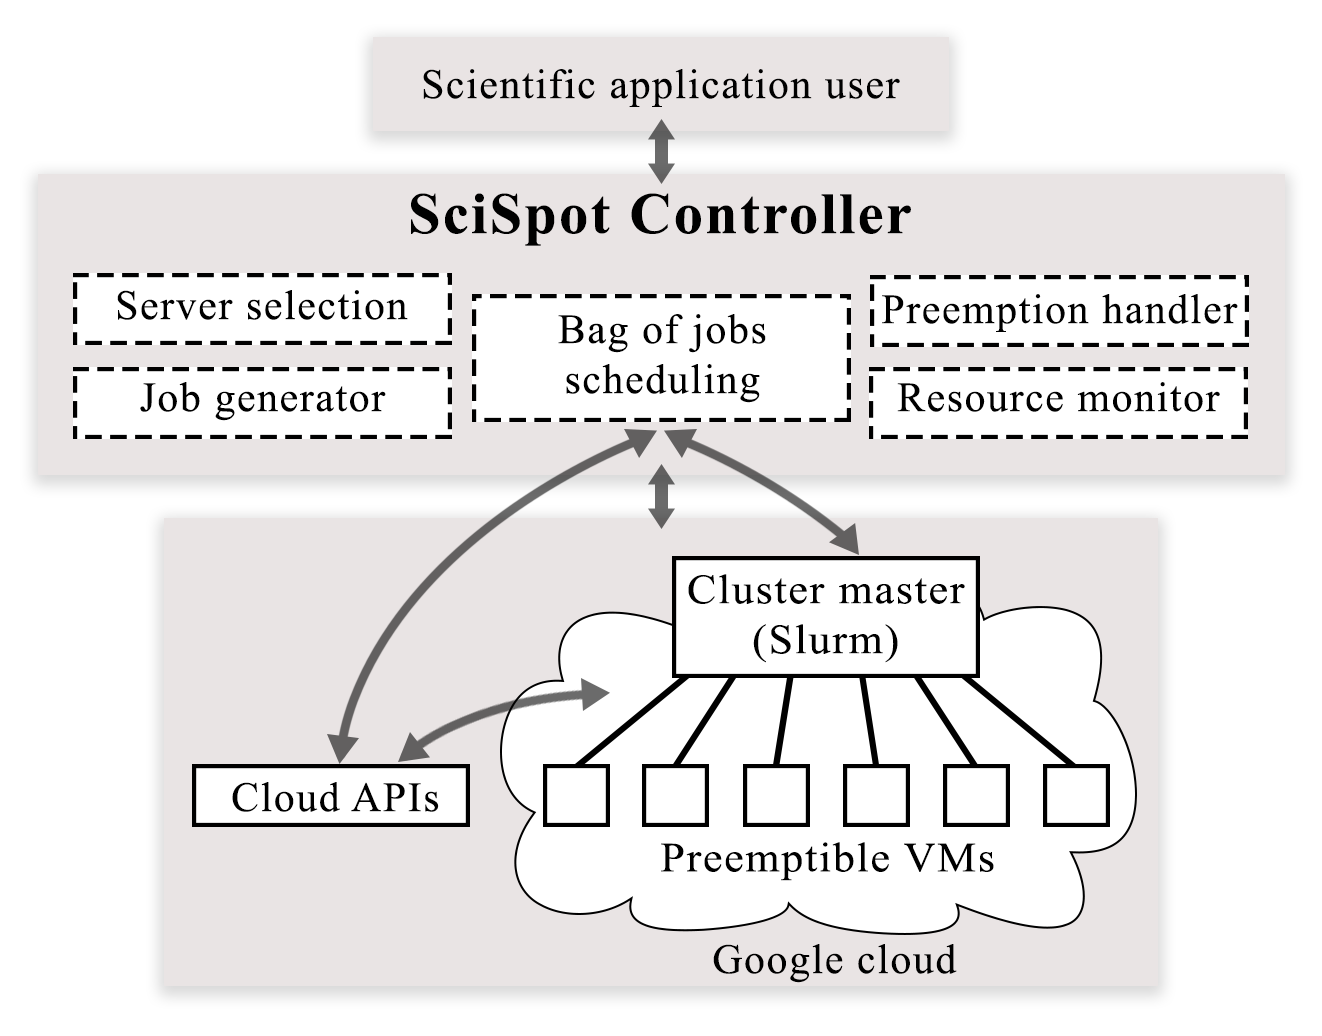
\includegraphics[width=0.3\textwidth]{../figures/Architecture.png}
  \caption{SciSpot Architecture}
  \label{fig:arch}
\end{figure}

\sysname aims to provide a simple user interface to allow users to deploy their applications with the a minimum changes to their workflow.
Most scientific applications are deployed on HPC clusters that have a cluster or a job manager such as Slurm~\cite{slurm} or Torque~\cite{torque}, and \sysname integrates with the cluster manager (e.g., Slurm) to provide the same interface to applications.
As shown in Figure~\ref{fig:arch}, \sysname creates and manages clusters of transient cloud servers, manages all aspects of the VM lifecycle and costs, and implements the various policies described in the rest of this section. 


\noindent \textbf{High-level work flow:} When a user wishes to run a bag of jobs, \sysname handles the provisioning of a cluster of transient cloud servers, and scheduling and monitoring of the bag of jobs, in addition to dealing with preemptions.
Execution of a bag of jobs proceeds in two phases. In the first phase, \sysname selects the ``right'' cluster configuration for a given application through a cost-minimizing exploration-based search policy, described next in Section~\ref{subsec:server-selection}.
In the second phase, \sysname proceeds to run the remaining jobs in the bag on the optimal cluster configuration. 

\subsection{Server Selection}
\label{subsec:server-selection}

\subsubsection{Why Server Selection is Necessary}

%\noindent \textbf{Why server selection is necessary:}
Before deploying any application on the transient cloud servers, we must first select the ``right'' cloud server for the application. 
Since cloud platforms support a wide range of applications, they also offer a large range of servers (VMs) with different resource configurations (such as the number of CPU cores, memory size, I/O bandwidths, etc.). 
For example, a cloud provider may offer VMs with (4 CPUs, 4 GB memory), (8 CPUs, 8 GB memory), etc.
Most clouds offer a large number of different hardware configurations---Amazon EC2 offers more than 50 hardware configurations, for example~\cite{amazon-ec2-instance-types}. 

\noindent \emph{Importantly, different server configurations have different cost, performance, and preemption characteristics. }

% Why crucial for parallel jobs

%Selecting for performance 
Even if we assume that the total amount of resources to be allocated to a job is fixed, there are multiple \emph{cluster configurations} to satisfy the allocation with the large number of available server types. 
For example, a job requiring a total of 128 CPUs can be run on a cluster of 2 servers with 64 CPUs each, or 4 servers with 32 CPUs each, etc. 
Server selection is especially important for parallel applications, because although the total amount of resources in each cluster configuration is constant, the resources are distributed differently. 
Since the performance of parallel applications is particularly sensitive to their communication overheads, different cluster configurations may yield different job running times.
For instance, a smaller cluster with large servers will result in lower inter-server communication, and thus lower running times. 

%Selecting for preemptibility 
However, the performance of an application is also affected by preemptions of transient servers.
Since preemptions are essentially fail-stop failures, synchronous parallel applications (such as those using MPI) are forced to abort, and completing the job requires restarting it.
Thus, preemptions can increase the overall running time of a job, with the increase in the job's running time determined by the frequency of preemptions.


\subsubsection{Server Selection Policy}

Having provided the motivation and tradeoffs in server selection, we now describe how \sysname's server selection policy. 
Given an application and a bag of jobs, \sysname ``explores'' and searches for the right server type by minimizing the expected cost of running the job.

We first determine the search space, which is the space of all cluster configurations $\langle i,n_i \rangle$ such that $r_i n_i = \mathcal{R}$. With $N$ server types, this results in at most $N$ cluster configurations.
Each configuration will yield different application performance, preemption overhead, and cost.
Our server selection policy runs the application on on each configuration to determine its running time (in the absence of preemptions), which is denoted by $T_{\langle i,n_i \rangle}$. 
\sysname thus does an exhaustive search over all valid cluster configurations to find the lowest-cost configuration $\langle i, n_i \rangle$. 

We note that this search is different from conventional speedup plots in which the objective is to determine the how well an application scales with increasing amount of resources and parallelism. 
In contrast, we \emph{fix} the total amount of resources allocated to the application's job ($=\mathcal{R}$), and only vary \emph{how} these resources are distributed, which affects communication overhead and hence the performance.
%Weak
We assume that the total resource requirement for a job, $\mathcal{R}$ can be easily provided by the user based on prior speedup data and the user's cloud budget and the deadline for job completion. 



\subsubsection{Server Cost Model}

Since server selection involves a tradeoff between cost, performance, and preemptions, we develop a model that allows us to optimize the resource allocation and pick the ``best'' server type that minimizes the expected cost of running an application on transient cloud servers. 


Let us assume that the cloud provider offers $N$ server types, with the price of a server type equal to $c_i$. 
Let $\mathcal{R}$ denote the total amount of computing resources requested for the job. For ease of exposition, let us assume that $\mathcal{R}$ is the total number of CPU cores.
Furthermore, let $r_i$ denote the ``size'' of the server of type $i$.
Then, the number of servers of type $i$ required, $n_i = \mathcal{R}/r_i$. 

The overall expected cost of running a job can then be expressed as follows:
\begin{equation}
  \label{eq:e-cost}
  E[C_{\langle i,n_i \rangle}] = n_i*c_i * E[T_{\langle i,n_i \rangle}]
\end{equation}
Here, $E[T_{\langle i,n_i \rangle}]$ denotes the expected running time of the job on $n_i$ servers of type $i$.
This running time, in turn depends on the preemption probability of the server type:
\begin{align}
  \label{eq:et1}
  E[T_{\langle i,n_i \rangle}] &= T_{\langle i,n_i \rangle} + E[\text{Recomputation Time}] \\
  &= T_{\langle i,n_i \rangle} + P(\text{at least one preemption})*T_{\langle i,n_i \rangle}/2   
\end{align}
Here, $T_{\langle i,n_i \rangle}$ is the running time of the job without failures, which we obtain empirically as explained in the previous subsection.

The probability that at least one VM out of $n_i$ will be preempted during the job execution can be expressed as:

\begin{align}
  \label{eq:pfail1}
  P(\text{at least one preemption}) &= 1-P(\text{no preemptions}) \\
                                 &= 1-(1-P(i, t))^{n_i} \\
                                 &= 1-\left(1-\dfrac{T_{\langle i,n_i \rangle}}{E[L_i]}\right)^{n_i}      
\end{align}

Here, $P(i, t)$ denotes the probability of a preemption of a VM of type $i$ when a job of duration $t$ runs on it. 

It depends on the type of server, and we use historically determined failure distributions.
In the expectation, it is given by:
\begin{equation}
  \label{eq:pi}
  P(i, t) = \dfrac{t}{E[L_i]}
\end{equation}
Where $E[L_i]$ is the expected lifetime of the VM of type $i$ as computed with through the analytical model in earlier section.
As a first order approximation, the running time of the job, $t=T_{\langle i,n_i \rangle}$, which is empirically obtained for a given application. 


Thus, we can see that if we select smaller VMs, we will require more of them (higher $n_i$), and this cluster configuration will have a larger probability of failure and thus higher running times and costs.
However, there is a tradeoff: selecting larger VMs results in smaller $n_i$, but larger VMs have higher preemption probability, as we have seen in Section~\ref{subsec:types-dynamics}. 



% Limiting the exploration search space
%\sysname thus explores the cluster configuration space to find empirical job running times, which depend on the application and it's parallel structure.
%We then use the analytically derived preemption probability to compute the expected running time, and finally the total expected cost.

To limit the search space, we observe that since most scientific applications are CPU bound, and we only need to consider VMs meant for CPU-bound workloads, such as \texttt{highcpu} VMs in Google Cloud and the \texttt{cc} family in Amazon EC2.
For example, the Google cloud offers a total of 7 \texttt{highcpu} server types with 1, 2, 4, 8, 16, 32, and 64 CPU's---yielding a small upper bound on the number of configurations to search. 
Furthermore, a large cluster of small servers is suboptimal for most applications (except those that are completely embarassingly parallel and have no communication).
\sysname thus explores VM's in descending order of their size and ignores exploring the small VMs (with 2 CPUs or fewer)---reducing the search space even further. 


%\sysname launches clusters of preemptible VMs during the exploration phase. 

\subsection{Scheduling a Bag of Jobs}


Once the right cluster configuration for a job has been determined, \sysname then proceeds to run the remaining jobs in the bag.
A bag of jobs is determined by the total number of jobs in the bag, associated parameters for each job, and the minimum number of jobs that must be successfully executed.  
Given these parameters as input, \sysname then creates a cluster by launching preemptible VMs and starts scheduling the different jobs in a bag.

\sysname also allows users to specify a deadline for bag completion, which we use to compute the number of jobs to execute in parallel. If the deadline specified is $D$, then the number of parallel jobs is $k=D/m*E[T]$. Thus if the exploration phase recommends $n_i$ VMs, then we launch a cluster of $k*n_i$ VMs, with each job executing on $n_i$ VMs. 
For this calculation, we assume that the running time of different jobs in a bag will largely be similar, but this is not a correctness requirement.
Thus because of the stochasticity in job running times and VM lifetimes, \sysname only meets the deadline in a ``best effort'' manner, and does not guarantee strict makespan constraints. 

Upon job completion, the next job in the bag is run. 
When a job fails due to VM preemption, \sysname replenishes the cluster by launching replacement VM's and resubmits the job. 
Jobs are restarted from a checkpoint if available.
We do not restart failed jobs as long as we can complete the minimum number of jobs in the bag.
Due to high demand, preemptible VM's of the chosen type may not be available.
In such cases, \sysname runs in a ``degraded'' mode---jobs are either run on a smaller number of VMs, or are run on VM's of a different size that are available but may have suboptimal cost.  



%Jobs in bag can either be explicitly supplied with parameters, or 



%We note that the jobs in the bags are for the same application, so their computational and communication complexity can be assumed to the same across the bag. 


%%%%%%%%%%%%%%%%%%%%%%%%%%%%%%%%%%%%%%%%%%%%%%%%%%


\begin{comment}

  Our server selection policy is empirical and black-box in nature in that we don't assume an application model.
However due to the bag of jobs execution model, we do not need to special pilot jobs, but the jobs for doing the profiling come from the bag itself.


Thus given a desired allocation, \sysname's server selection policies select the ``best'' server type for a given application. 

One of key characteristics of transient cloud computing is the heterogeneity and diversity in the server configurations offered by most cloud platforms. 
Different configurations or types of servers have different prices 

\end{comment}



%%% Local Variables:
%%% mode: latex
%%% TeX-master: "paper"
%%% End:


%\section{Checkpointing Policies}

High rate of failure means that especially for long jobs, checkpointing is necessary.
In this section, we develop checkpointing policies.

At a high level, we only checkpoint long jobs, based on the probability of preemption.

Once checkpointing for a job is enabled, we use proactive periodic checkpointing.

DMTCP is used for checkpointing MPI programs.

Conventionally, periodic checkpointing according to Young-Daly formula: $\tau=\sqrt{2\cdot\delta\cdot\text{MTTF}}$.
This assumes that failure arrival process is exponentially distributed.

However, this may not always hold true.
Clearly, from Figure 1, the CDF is not exponential.

Much more strongly ``bath-tub''. Maybe can use exponentiated Weibull to model the failures.

Regardless, because it is not memoryless, the checkpointing interval cannot be uniform. Maybe can use~\cite{bougeret_checkpointing_2011}, which uses dynamic programming and also comes with a simulator of sorts. 




%%% Local Variables:
%%% mode: latex
%%% TeX-master: "paper"
%%% End:


%\vspace*{\subsecspace}
%\section{SciSpot Design and Implementation}
\subsection{Details of the Experimental Framework used for Evaluation}
%\section{Model-Informed Policy Implementation}
\label{sec:impl}


\sysname is a general-purpose software framework for running scientific computing applications on low-cost transient cloud servers.
It incorporates policies and mechanisms for generating, deploying, orchestrating, and monitoring bags of jobs on cloud servers.
Specifically, it runs a bag of jobs defined by these parameters:
\begin{lstlisting}[basicstyle=\sffamily, frame=single, columns=fullflexible, escapeinside={(*}{*)}]
  Bag of job = {(*$\mathcal{A}$*): Application to execute,
  (*$n$*): Number of jobs,
  (*$m$*): Minimum number of jobs to finish,
  (*$\pi$*): Generator function for job parameters,
  (*$\mathcal{R}$*): Computing resources per job}
\end{lstlisting}


%Additionally, ease-of-use is one of \sysname's primary design goals, and we specifically incorporate

%it is suitable for running a large variety of applications.
\sysname seeks to minimize the cost and running time of bags of jobs of scientific computing applications.
\sysname's cost and time minimizing policies for running bags of jobs are based on empirical and analytical models of the cost and preemption dynamics of  transient cloud servers, which we present in the next section. 

\sysname is designed as a framework that increases the usability and viability of transient cloud servers for scientific computing applications, and provides a simple user interface to allow users to deploy their applications with minimum workflow changes. 
Most scientific computing applications are deployed on HPC clusters that have a batch scheduler such as Slurm~\cite{slurm} or Torque~\cite{torque}, and \sysname integrates with these schedulers (e.g., Slurm) to provide the same interface to applications. 
As shown in Figure~\ref{fig:arch},
\sysname creates and manages clusters of transient cloud servers, manages all aspects of the VM lifecycle and costs, and implements the various policies described in the rest of this section. 

\begin{figure}[t]
  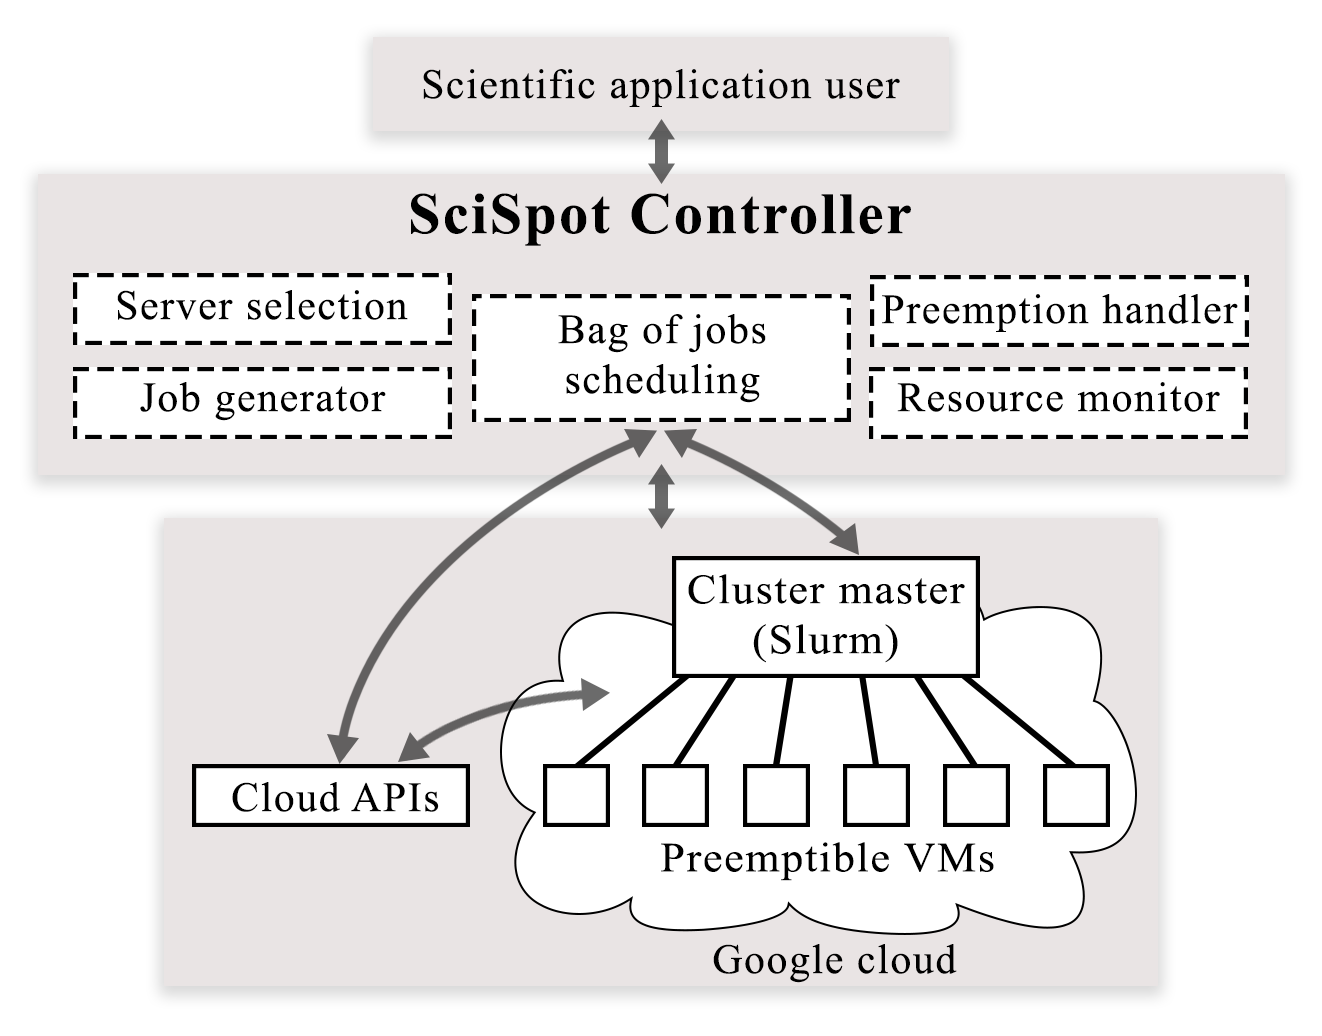
\includegraphics[width=0.3\textwidth]{../figures/Architecture.png}
\vspace*{\myfigspace}
  \caption{SciSpot architecture and system components.}
  \label{fig:arch}
  \vspace*{\myfigspace}
\end{figure}


\noindent \textbf{High-level workflow:} When a user wishes to run a bag of jobs, \sysname handles the provisioning of a cluster of transient cloud servers.
In addition, \sysname deals with the scheduling and monitoring of the bag of jobs, and with VM preemptions. 
Execution of a bag of jobs proceeds in two phases.
In the first phase, \sysname selects the ``right'' cluster configuration for a given application through a cost-minimizing exploration-based search policy, described in Section~\ref{subsec:server-selection}. 
In the second phase, \sysname proceeds to run the remaining jobs in the bag on the optimal cluster configuration. 

\prat{End design}


\sysname is implemented as a light-weight, extensible framework that makes it convenient and cheap to run scientific computing applications in the cloud.
We have implemented the \sysname prototype in Python in about 2,000 lines of code, and currently support running VMs on the Google Cloud Platform~\cite{gcp}. 
%
\sysname is implemented as a centralized controller, which implements the VM selection and job scheduling policies described in Section~\ref{sec:design}. 
The controller can run on any machine (including the user's local machine, or inside a cloud VM), and exposes an HTTP API to end-users. 
Users submit bags of jobs to the controller via the HTTP API, which then launches and maintains a cluster of cloud VMs, and maintains the job queue and metadata in a local database. 
To improve usability, we automatically generate parameter combinations for a given bag size, based on a user-provided json file with ranges and constraints for each parameter. 

\sysname integrates, and interfaces with two primary services.
First, it uses the Google cloud API~\cite{gcloud-api} for launching, terminating, and monitoring VMs.
Once a cluster is launched, it then configures a cluster manager such as Slurm~\cite{slurm} or Torque~\cite{torque}, to which it submits jobs. 
\sysname uses the Slurm cluster manager, with each VM acting as a Slurm ``cloud'' node, which allows Slurm to gracefully handle VM preemptions.
The Slurm master node runs on a small, 2 CPU non-preemptible VM, which is shared by all applications and users. 
\sysname monitors job completions and failures (due to VM preemptions) through the use of Slurm call-backs, which issue HTTP requests back to the \sysname controller.

%As part of \sysname, we also provide a base VM image with Slurm and MPI integration, along with commonly used libraries and benchmarks for scientific computing. To run an application, users must provide a location to the application source code or binaries. Integrating \sysname with container-based image management tools such as Docker~\cite{docker} and Singularity~\cite{kurtzer2017singularity} is part of our ongoing work. 





%%% Local Variables:
%%% mode: latex
%%% TeX-master: "paper"
%%% End:


\vspace*{\subsecspace}
%\section{Experimental Evaluation}
%\section{Model Testing and Validation}
%\section{Testing and Evaluation of Model-Informed Policies}
\section{Model and Policy Evaluation}
\label{sec:eval}

%%\vspace*{\subsecspace}
%\section{SciSpot Design and Implementation}
\subsection{Details of the Experimental Framework used for Evaluation}
%\section{Model-Informed Policy Implementation}
\label{sec:impl}


\sysname is a general-purpose software framework for running scientific computing applications on low-cost transient cloud servers.
It incorporates policies and mechanisms for generating, deploying, orchestrating, and monitoring bags of jobs on cloud servers.
Specifically, it runs a bag of jobs defined by these parameters:
\begin{lstlisting}[basicstyle=\sffamily, frame=single, columns=fullflexible, escapeinside={(*}{*)}]
  Bag of job = {(*$\mathcal{A}$*): Application to execute,
  (*$n$*): Number of jobs,
  (*$m$*): Minimum number of jobs to finish,
  (*$\pi$*): Generator function for job parameters,
  (*$\mathcal{R}$*): Computing resources per job}
\end{lstlisting}


%Additionally, ease-of-use is one of \sysname's primary design goals, and we specifically incorporate

%it is suitable for running a large variety of applications.
\sysname seeks to minimize the cost and running time of bags of jobs of scientific computing applications.
\sysname's cost and time minimizing policies for running bags of jobs are based on empirical and analytical models of the cost and preemption dynamics of  transient cloud servers, which we present in the next section. 

\sysname is designed as a framework that increases the usability and viability of transient cloud servers for scientific computing applications, and provides a simple user interface to allow users to deploy their applications with minimum workflow changes. 
Most scientific computing applications are deployed on HPC clusters that have a batch scheduler such as Slurm~\cite{slurm} or Torque~\cite{torque}, and \sysname integrates with these schedulers (e.g., Slurm) to provide the same interface to applications. 
As shown in Figure~\ref{fig:arch},
\sysname creates and manages clusters of transient cloud servers, manages all aspects of the VM lifecycle and costs, and implements the various policies described in the rest of this section. 

\begin{figure}[t]
  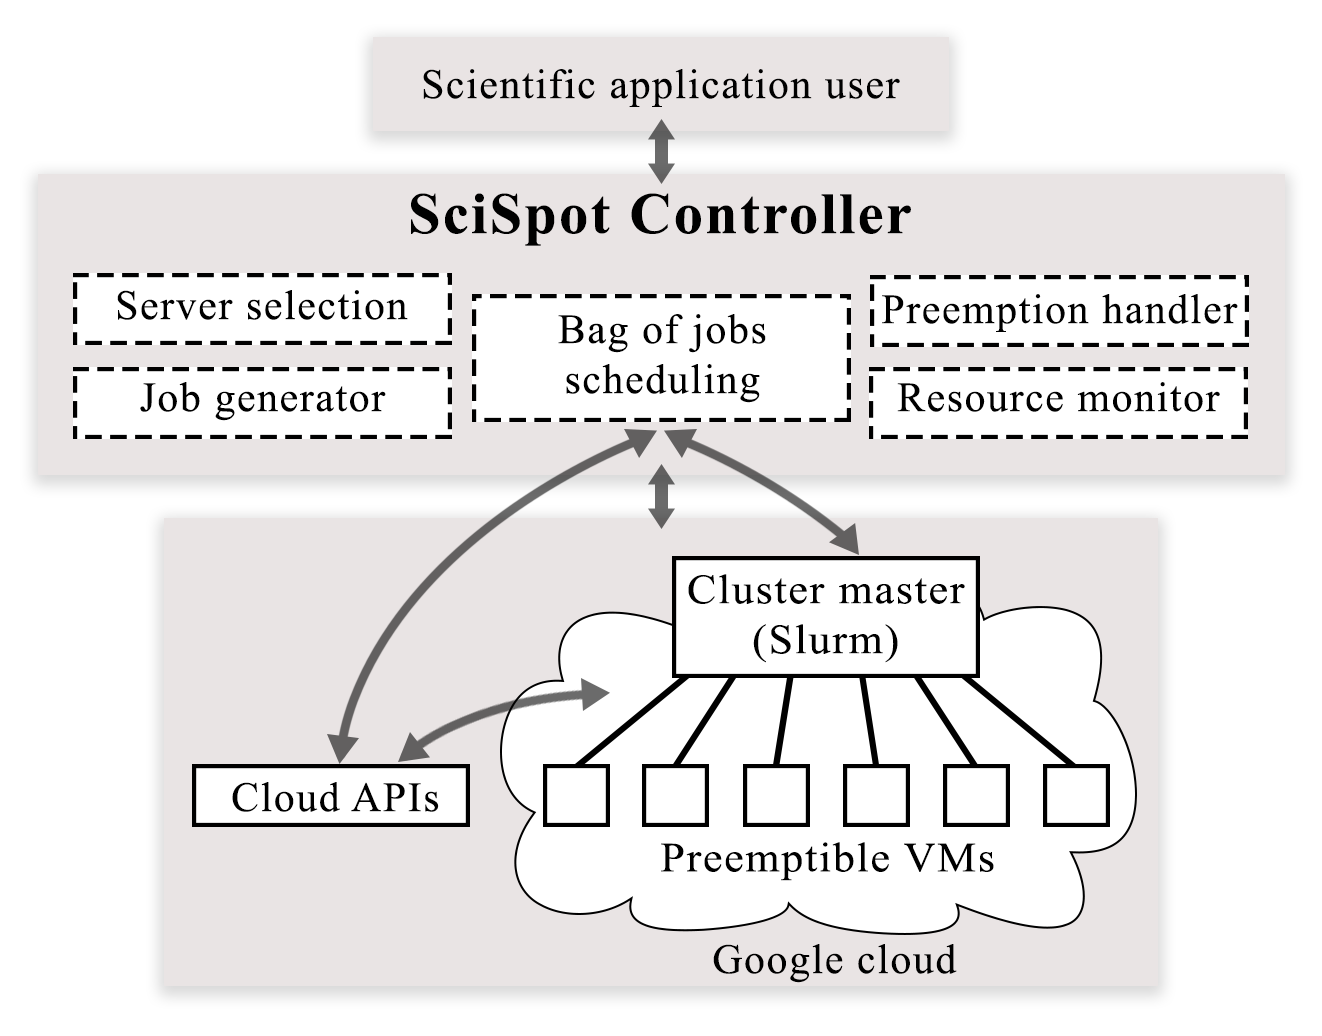
\includegraphics[width=0.3\textwidth]{../figures/Architecture.png}
\vspace*{\myfigspace}
  \caption{SciSpot architecture and system components.}
  \label{fig:arch}
  \vspace*{\myfigspace}
\end{figure}


\noindent \textbf{High-level workflow:} When a user wishes to run a bag of jobs, \sysname handles the provisioning of a cluster of transient cloud servers.
In addition, \sysname deals with the scheduling and monitoring of the bag of jobs, and with VM preemptions. 
Execution of a bag of jobs proceeds in two phases.
In the first phase, \sysname selects the ``right'' cluster configuration for a given application through a cost-minimizing exploration-based search policy, described in Section~\ref{subsec:server-selection}. 
In the second phase, \sysname proceeds to run the remaining jobs in the bag on the optimal cluster configuration. 

\prat{End design}


\sysname is implemented as a light-weight, extensible framework that makes it convenient and cheap to run scientific computing applications in the cloud.
We have implemented the \sysname prototype in Python in about 2,000 lines of code, and currently support running VMs on the Google Cloud Platform~\cite{gcp}. 
%
\sysname is implemented as a centralized controller, which implements the VM selection and job scheduling policies described in Section~\ref{sec:design}. 
The controller can run on any machine (including the user's local machine, or inside a cloud VM), and exposes an HTTP API to end-users. 
Users submit bags of jobs to the controller via the HTTP API, which then launches and maintains a cluster of cloud VMs, and maintains the job queue and metadata in a local database. 
To improve usability, we automatically generate parameter combinations for a given bag size, based on a user-provided json file with ranges and constraints for each parameter. 

\sysname integrates, and interfaces with two primary services.
First, it uses the Google cloud API~\cite{gcloud-api} for launching, terminating, and monitoring VMs.
Once a cluster is launched, it then configures a cluster manager such as Slurm~\cite{slurm} or Torque~\cite{torque}, to which it submits jobs. 
\sysname uses the Slurm cluster manager, with each VM acting as a Slurm ``cloud'' node, which allows Slurm to gracefully handle VM preemptions.
The Slurm master node runs on a small, 2 CPU non-preemptible VM, which is shared by all applications and users. 
\sysname monitors job completions and failures (due to VM preemptions) through the use of Slurm call-backs, which issue HTTP requests back to the \sysname controller.

%As part of \sysname, we also provide a base VM image with Slurm and MPI integration, along with commonly used libraries and benchmarks for scientific computing. To run an application, users must provide a location to the application source code or binaries. Integrating \sysname with container-based image management tools such as Docker~\cite{docker} and Singularity~\cite{kurtzer2017singularity} is part of our ongoing work. 





%%% Local Variables:
%%% mode: latex
%%% TeX-master: "paper"
%%% End:


%Opening is deliberately short because we gonna be running out of space

In this section, we present analytical and empirical evaluation of constrained preemptions.
We have already presented the statistical analysis of our model in Section~\ref{sec:failmodel}, and we now focus on answering the following questions: 

\begin{enumerate}
\item How do constrained preemptions impact the total running time of applications?

\item  What is the effect of our model-based policies when compared to existing transient computing approaches?

%\item What is the real-world cost and performance of running batch applications?

\item What is the cost and performance of our batch computing service for real-world workloads? 
  
\end{enumerate}




\noindent \textbf{Environment and Workloads:}
All our empirical evaluation is conducted on the Google Public cloud using our batch computing service described in the previous section. 
We use three scientific computing workloads that are representative of typical applications in the broad domains of physics, material sciences, and chemical engineering:

% open-source
%\vspace*{\tightext}
%\begin{description}
  %TODO: Need MAX two sentence descriptions

\noindent \textbf{Nanoconfinement.}
The nanoconfinement application launches molecular dynamics (MD) simulations of ions in nanoscale confinement created by material surfaces \cite{jyto,kadupitiya2017}.

\noindent \textbf{Shapes.} The Shapes application runs an MD-based optimization dynamics to predict the optimal shape of deformable, charged nanoparticles \cite{jto1,jjzo1}. 

\noindent \textbf{LULESH.} Livermore Unstructured Lagrangian Explicit Shock Hydrodynamics (LULESH)  is a popular benchmark for hydrodynamics simulations of continuum material models \cite{IPDPS13:LULESH,LULESH2:changes}. 
% \end{description}

% These examples are representative of typical scientific computing applications in the broad domain of physics, materials science, and chemical engineering. These three examples are implemented as parallel programs that use OpenMP and MPI parallel computing techniques. The first two are used in nanoscale materials research \cite{jso1,jso2,solis2013generating,jjzo1,jto1,jyto} and LULESH is a widely used benchmark \cite{IPDPS13:LULESH,LULESH2:changes}.

%All applications are run with default parameters unless otherwise stated.




\subsection{Impact of Constrained Preemptions on Job Running Times}

\begin{figure}[t]
  \subfloat[Computation wasted due to one preemption. \label{fig:vs-uniform}]
  {  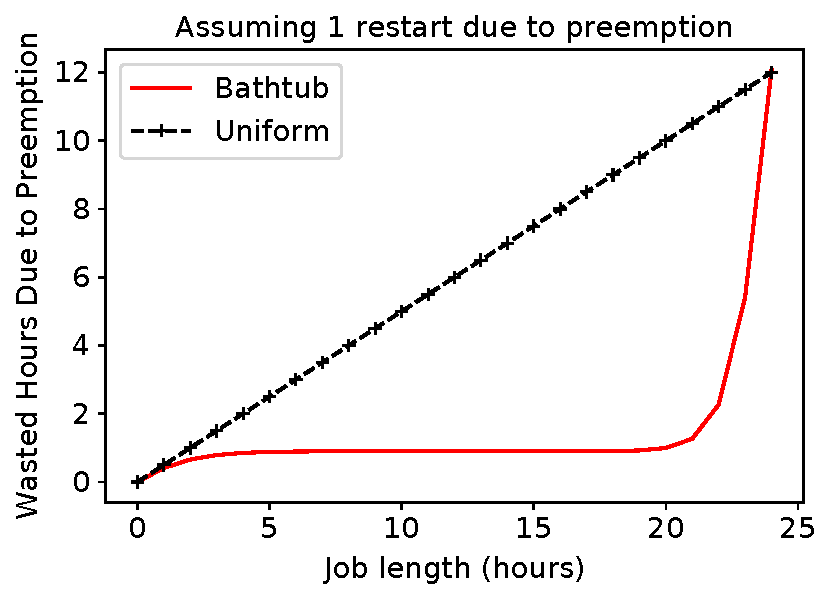
\includegraphics[width=0.3\textwidth]{../graphs/uniform-v-bathtub.pdf} }
  \\
    \subfloat[Expected increase in running time. \label{fig:vs-uniform-2}]
    {  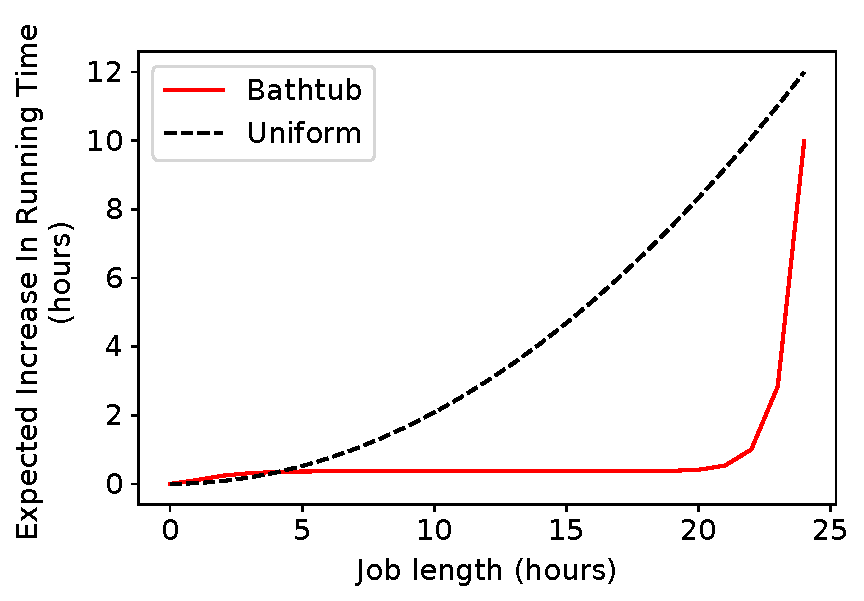
\includegraphics[width=0.3\textwidth]{../graphs/uniform-v-bathtub-2.pdf} }
    \caption{Wasted computation and expected increase in running time for uniform vs. baththub failures. For jobs $>5$ hours, bathtub distribution results in significantly lower wasted computation.}
  \label{fig:vs-uniform-both}
  
\end{figure}

%\caption{The expected wasted computation, given a single failure, is lower when preemptions are distributed in a bathtub shape, compared to uniformly distributed over the 24 hour interval}

We begin by examining how constrained preemptions impacts the total job running times. 
When a preemption occurs during the job's execution, it results in wasted work, assuming there is no checkpointing. 
This increases the job's total expected running time, since it must restart after a preemption.
In case of constrained preemptions, the expected waste depends both on the probability of job preemption, as well as \emph{when} the job was preempted. 


For a job of length $J$, the wasted work, assuming that the job faces a \emph{single} preemption, is $E[W_1(J)]$, and is given by Equation~\ref{eq:wasted}.
We first analyze this wasted work for jobs of different lengths in Figure~\ref{fig:vs-uniform}
We analyze two failure probability distributions for constrained preemptions: a uniform distribution such that $F(t) = 24-t$, and the bathtub shaped distribution with parameters corresponding to the \texttt{n1-highcpu-16} VM type shown in Figure~\ref{fig:gcp1}. 


For the uniform distribution, the wasted work is linear in the job length, and is given by $J/2$.
For the bathtub distribution, the wasted work is given by Equation~\ref{eq:wasted}, and is \emph{significantly} lower, especially for longer jobs (longer than 5 hours). 
With the bathtub distribution, jobs see a high rate of failure initially, but that also reduces the wasted work. 
Once jobs survive the initial high failure rate, the rate of failure is low, and thus the wasted work is more or less constant for all but the shortest and longest jobs. 



We now examine the expected increase in running time, that also accounts for the probability of failure, and is given by $P(\text{failure})*E[W_1]$. 
Figure~\ref{fig:vs-uniform-2} shows this expected increase in running times for jobs of different lengths.
We see that for uniformly distributed preemptions, the increase in running time is quadratic in the job length (and is given by $J^2/48$).
Interestingly, the high rate of early failures for the bathtub distribution results in a slightly worse (i.e., higher) running time for short jobs.
However for jobs longer than 5 hours, a cross-over point is reached, and the bathtub distribution provides a significantly lower overhead of preemptions. 
For instance, for a 10 hour job, the increase in running time is about 30 minutes, or 5\%. 
In contrast, if failures were uniformly distributed, the increase would be 2 hours. 


Thus, the bathtub preemptions are beneficial for applications and users, as the low failure rate during the middle periods results in significantly lower wasted work, compared to the uniformly distributed failures.
Since the failure rate distribution is ultimately controlled by the cloud provider, our analysis can be used to determine the appropriate distribution based on the job length distributions.
For instance, if short jobs are very common, then uniformly distributed preemptions are preferable, otherwise, bathtub distributions can offer significant benefits. 

\noindent \textbf{Result:} \emph{For constrained preemptions, bathtub distributions significantly reduce the expected increase in running times for medium to long running jobs, but are slightly inferior for short jobs.}




%%%%%%%%%%%%%%%%%%%%%%%%%%%%%%%%%%%%%%%%%%%%%%%%%%%%%%%%%%%%%%%%%%%%%%
\subsection{Model-based Policies}
\label{subsec:eval-policy}

We now evaluate the effectiveness of model-driven policies that we proposed earlier in Section~\ref{sec:policies}.
Specifically, we seek to compare the effectiveness of our job scheduling and checkpointing policies with existing transient computing approaches.



\subsubsection{Job Scheduling}

In the previous subsection, we have quantified the increase in running time due to preemptions, but we had assumed that jobs start on a newly launched server.
In many scenarios however, a server may be used for running a long-running sequence of jobs, such as in a batch-computing service. 
%
Our job scheduling policy is model-driven and decides whether to request a new VM for a job or run it on an existing VM.
A new VM may be preferable if the job starts running near the VM's 24 hour preemption deadline.
%However, since new VMs have a high initial rate of failure, we must be judicious 

Figure~\ref{fig:sched-bathtub} shows the effect of our job scheduling policy for a six hour job, for different job starting times (relative to the VM's starting time). 
We compare against a baseline of memoryless job scheduling that is not informed by constrained preemption dynamics.
Such memoryless policies are the default in existing transient computing systems such as SpotOn~\cite{spoton}. 
In the absence of insights about bathtub preemptions, the memoryless policy continues to run jobs on the existing VM. 
As the figure shows, the empirical job failure probability is bathtub shaped. 
However since the job is 8 hours long, with the memoryless policy, it will always fail when launched after $24-6=18$ hours.
In contrast, our model-based policy determines that after 18 hours, we will be better off running the job on a newer VM, and results in a much lower job failure probability (=0.4).
Thus, our model-based job scheduling policy can reduce job failure probability by taking into account the time-varying failure rates of VMs, which is not considered by existing systems that use memoryless scheduling policies.


\begin{figure}[t]
  \subfloat[Effect of job start time on the failure probability. \label{fig:sched-bathtub}]
  {  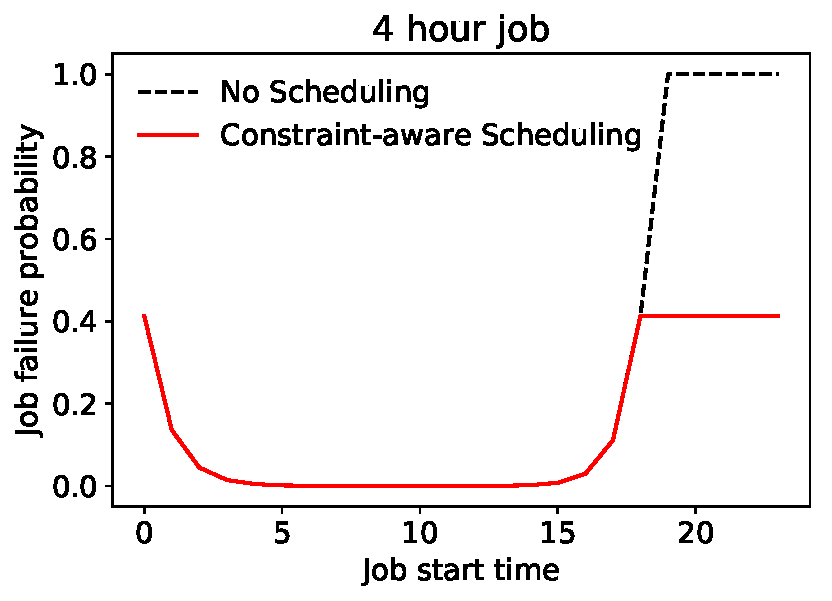
\includegraphics[width=0.35\textwidth]{../graphs/Sched-bathtub.pdf}}
  \\
  \subfloat[Job failure probability for jobs of different lengths. \label{fig:sched-all}]
  {  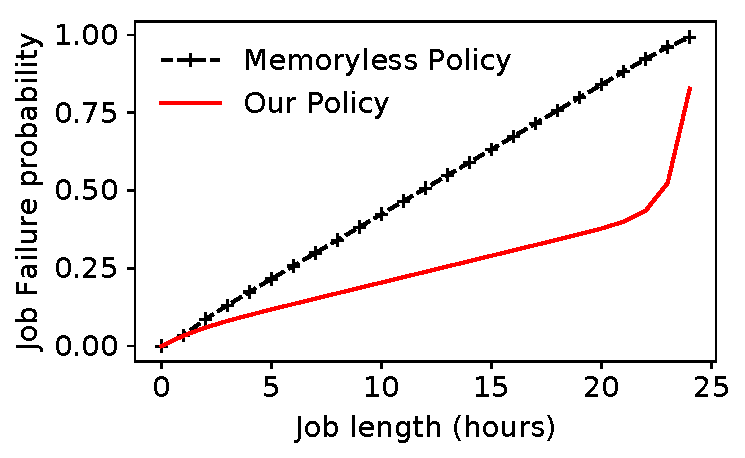
\includegraphics[width=0.35\textwidth]{../graphs/Sched-fail-prob.pdf}}
  \caption{Job failure probability is lower with our deadline aware policy across all job sizes.}
  \label{fig:sched-both}
\end{figure}

The job failure probability is determined by the job length and the job starting time.
We examine the failure probability for jobs of different lengths in Figure~\ref{fig:sched-all}, in which we average the failure probability across different start times.
We again see that our policy results in significantly lower failure probability compared to memoryless scheduling.
For all but the shortest and longest jobs, the failure probability with our policy is \emph{half} of that of existing memoryless policies.
This difference is primarily due to the differences in how the two policies perform for jobs launched near the end of the VM preemption deadline, which we examined previously in Figure~\ref{fig:sched-bathtub}. 


\noindent \textbf{Result:} \emph{Our model-based job scheduling and VM-reuse policy can decrease job failure probability by $2\times$.}



%%%%%%%%%%%%%%%%%%%%%%%%%%%%%%%%%%%%%%%%%%%%%%%%%%
\subsubsection{Checkpointing}
\label{subsec:eval-ckpt}

We now evaluate our model-based checkpointing policy, that uses a dynamic programming approach.
With our policy, the checkpointing rate is determined by the VM's current failure rate.
In contrast, all prior work in transient computing and most prior work in fault-tolerance assumes that failures are exponentially distributed (i.e., memoryless), and use the Young-Daly checkpointing interval.
In the Young-Daly approach, checkpoints are taken after a constant period given by $\tau \propto \sqrt{MTTF}$.
However in the case of constrained preemptions with bathtub distributions, the failure rate is time-dependent and not memoryless. 


The expected increase in running time for a 4 hour job is shown in Figure~\ref{fig:ckpt-4}, in which we account for both the increase due to the checkpointing overhead, as well as the expected recomputation due to preemptions. 
Throughout, we assume that each checkpoint takes 1 minute. 
The increase in running time depends on the failure rate and thus the job's starting time. 
With our model-based checkpointing policy, the increase in running time is bathtub shaped and is below 5\%, and around 1\% when the job is launched when the VM is between 5 and 15 hours old. 

We also compare with the Young-Daly periodic checkpointing policy, and use the initial failure rate of the VM to set the MTTF, which corresponds to an MTTF of 1 hour. 
This results in a high, constant rate of checkpointing, and thus increases the running time of the job by more than 25\%.
The increase in running time is primarily due to the overhead of checkpointing. 
Note that checkpointing with a lower frequency decreases the checkpointing overhead, but increases the recomputation required.

Next, we examine the expected running time of jobs of different length, when all jobs start at time=0, i.e, are launched on a freshly launched VM. 
Figure~\ref{fig:ckpt-start-0-relative} shows the expected increase in the running time of the jobs with our model-based checkpointing policy and the Young-Daly policy with MTTF=1 hour.
With our policy, the running times increase by 10\% for short jobs less than 2 hours long, and increase by less than 5\% for longer jobs.
In contrast, the Young-Daly policy yields a constant increase in running times of 25\%. 
Thus, our model-based policy is able to reduce the checkpointing overhead and thus reduce the performance overhead of running on preemptible VMs to below 5\%. 

\noindent \textbf{Result:} \emph{Our checkpointing policy can reduce the performance overhead of preemptions to under 5\%, which is $5\times$ better than conventional Young-Daly policies.}


\begin{figure}[t]
  \subfloat[Checkpointing overhead for different job starting times. \label{fig:ckpt-4}]
{  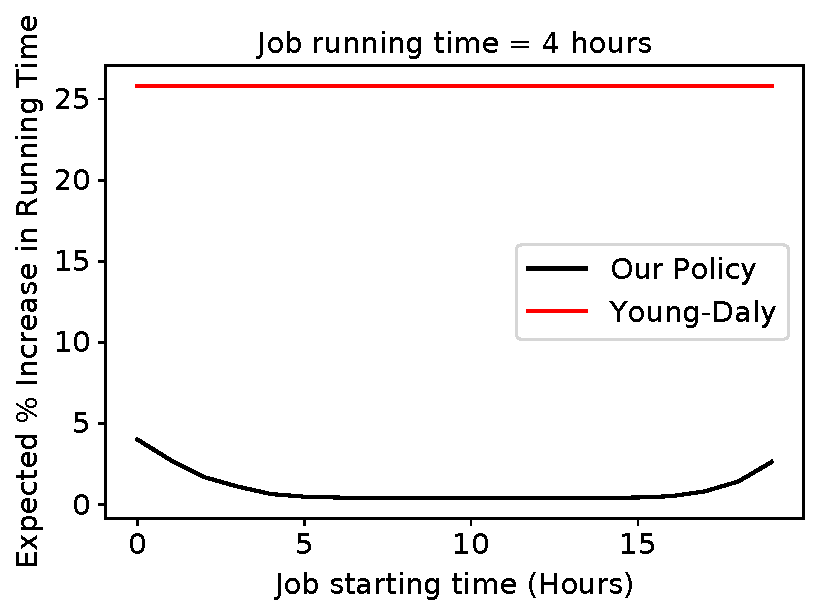
\includegraphics[width=0.35\textwidth]{../graphs/ckpt-4.pdf} }
%\hfill
% \subfloat[Running time with checkpointing when jobs start at time=0. \label{fig:ckpt-start-0}]
% {  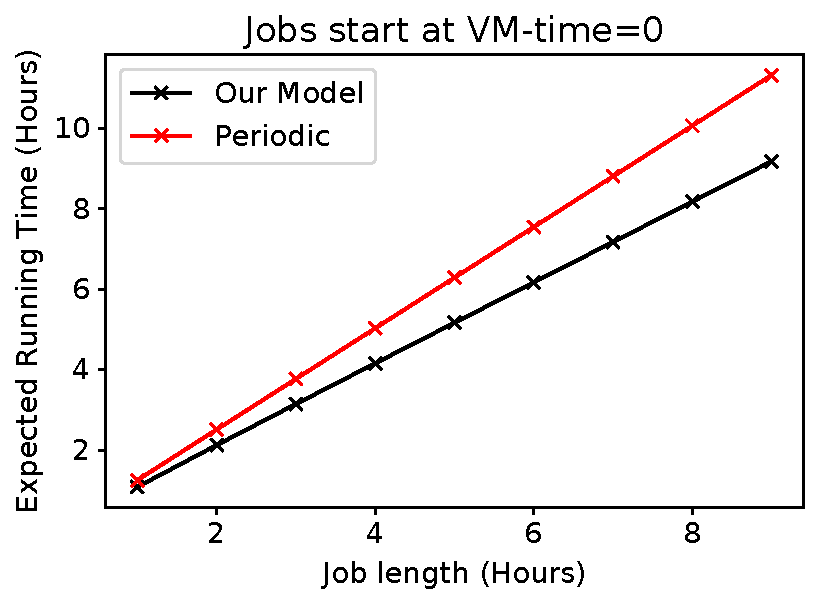
\includegraphics[width=0.3\textwidth]{../graphs/ckpt-start-0.pdf}}
% \hfill
\\
\subfloat[Increase in running time with checkpointing when jobs start at time=0. \label{fig:ckpt-start-0-relative}]
{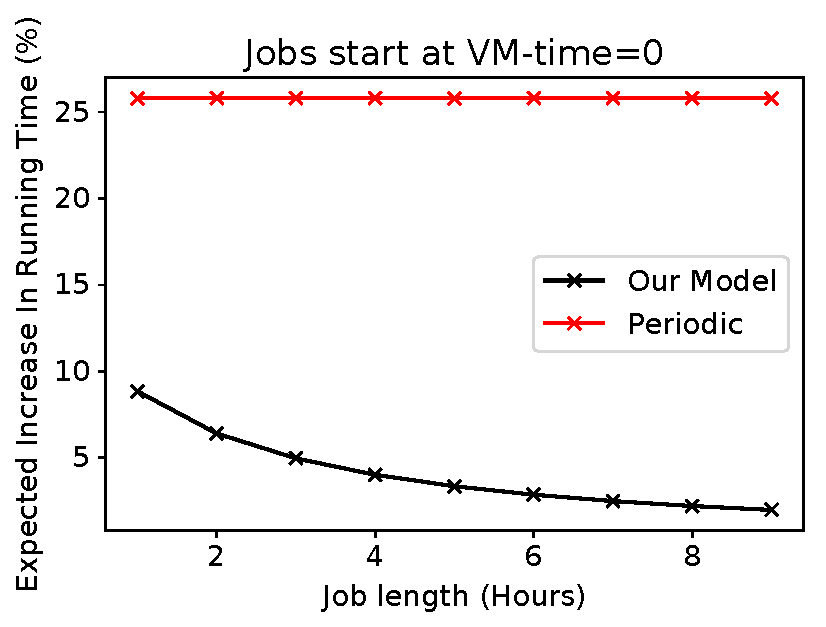
\includegraphics[width=0.35\textwidth]{../graphs/ckpt-start-relative.pdf}}

  \caption{Checkpointing effectiveness.}
  \label{fig:ckpt-all}
\end{figure}


%%%%%%%%%%%%%%%%%%%%%%%%%%%%%%%%%%%%%%%%%%%%%%%%%%

%\subsection{SciSpot Evaluation}
\subsection{Effectiveness on Scientific Computing Workloads}

We now show the effectiveness of our batch computing service on Google Preemptible VMs.
We run scientific simulation workloads described earlier in this section, and are interested in understanding the real-world effectiveness of our model-based service.
We use our model-driven job scheduling policy, but do not use checkpointing, since it requires additional 

%%%%%%%%%%%%%%%%%%%%%%%%%%%%%%%%%%%%%%%%%%%%%%%%%%


%As described in Section~\ref{sec:design}, applications can be deployed on multiple types of VMs in the cloud, with each VM type having a different ``size''.
%In our evaluation of parallel scientific computing applications that are CPU intensive, we are primarily interested in the number of CPUs in a VM.


%%%%%%%%%%%%%%%%%%%%%%%%%%%%%%%%%%%%%%%%%%%%%%%%%%


\begin{figure}[t]
  \centering
  \subfloat[Cost \label{fig:cost-only-bar}]
{  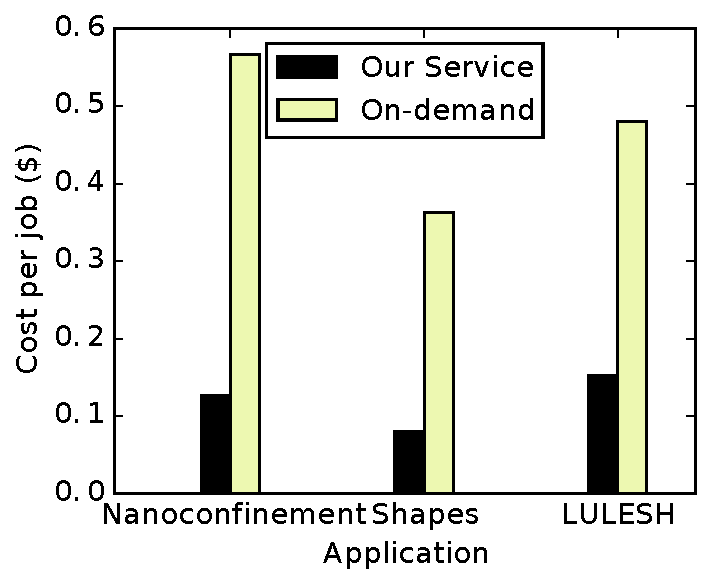
\includegraphics[width=0.25\textwidth]{../graphs/cost-vs-ondem.pdf} }
\hfill
\subfloat[Preemptions \label{fig:fails-time}]
{ 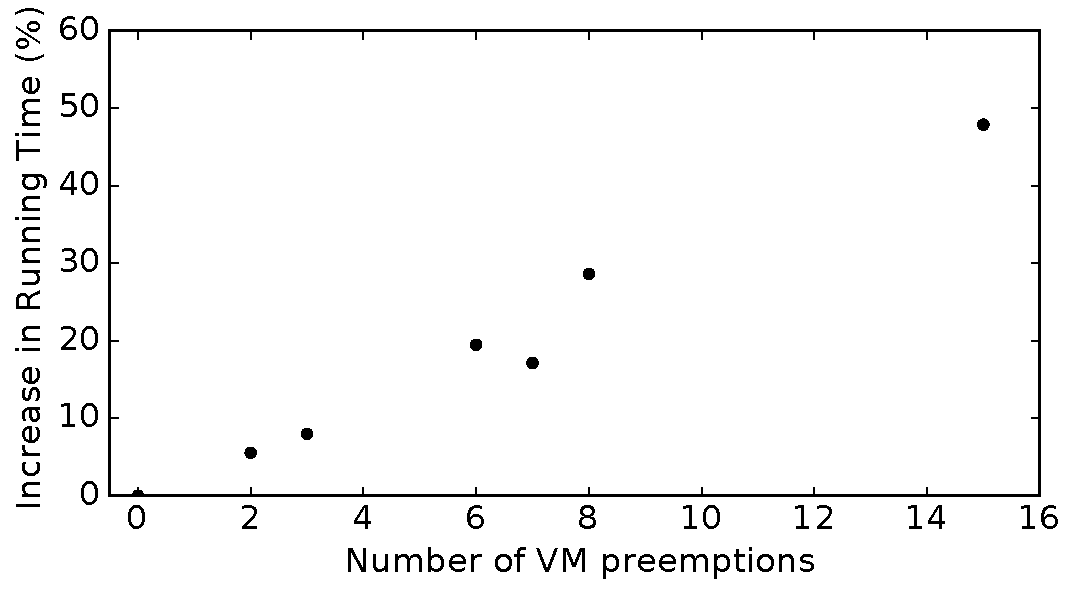
\includegraphics[width=0.2\textwidth]{../graphs/confin-fails-vs-time-relative.pdf} }
\label{fig:service-all}
\caption{Cost and preemptions with our service.}
\end{figure}  

%  \caption{SciSpot's use of preemptible VMs can reduce costs by up to $5\times$ compared to conventional cloud deployments, and 20\% compared to the state of the art EC2 spot instance selection (ExoSphere~\cite{exosphere}).}
%  \label{fig:cost-only-bar}
%    \vspace*{\myfigspace}


\noindent \textbf{Cost:}
The primary motivation for using preemptible VMs is their significantly lower cost compared to conventional ``on-demand'' cloud VMs that are non-preemptible.
To evaluate the cost of using our batch computing service, we run a bag of 100 jobs, all running on a cluster of 32 VMs of type \texttt{n1-highcpu-32}. 
Within a bag, different jobs are exploring different physical parameters, and job running times show little variance. 
Figure~\ref{fig:cost-only-bar} shows the cost of using Preemptible VMs compared to conventional on-demand VMs.
We see that for all the three applications, using our service can reduce costs by $5\times$.

We note that for this experiment, our  service was using model-driven job scheduling, but was not using checkpointing, since the applications lacked checkpointing mechanisms.
However, incorporating checkpointing would reduce the costs even further, since it would reduce the increase in running time (and server costs) due to recomputation.


\noindent \textbf{Preemptions:} 
Finally, we examine the effect of preemptions on the increase in running time under real-world settings.
We ran a cluster of 32 \texttt{n1-highcpu-32} VMs running the Nanoconfinement application, and repeated the experiment multiple times to observe the effect of preemptions.
Figure~\ref{fig:fails-time} shows the increase in running time of the entire bag of jobs, when different number of VM preemptions are observed during the entire course of execution.
We see that the net impact of preemptions results in a roughly linear increase in running time. 
Each preemption results in a roughly 3\% increase in running time, which validates our analytical evaluation shown earlier in Figure~\ref{fig:vs-uniform-2}.
The result also highlights the effectiveness of the job scheduling and VM-reuse policy, since most jobs run on the stable VMs, and  those that run on new VMs ``fail fast'' and result in only a small amount of wasted work and increase in running time. 


% \begin{figure}[t]
%   \centering 
%         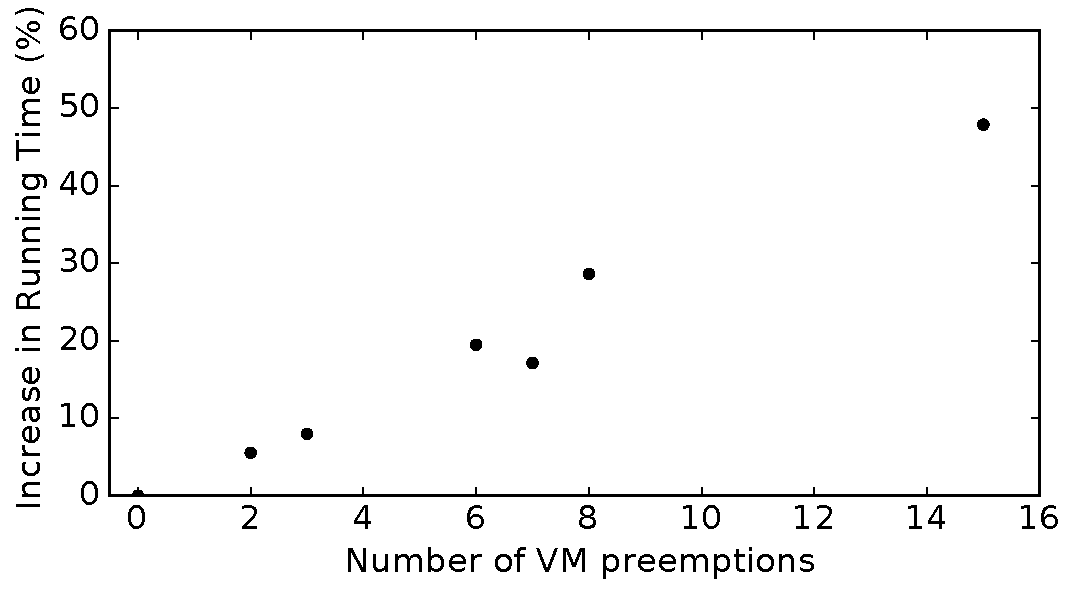
\includegraphics[width=0.22\textwidth]{../graphs/confin-fails-vs-time-relative.pdf}
%       \caption{The increase in running time due to preemptions is under 50\%, even at high preemption rates.}
%         %when the number of preemptions is high.}
%   \label{fig:fails-time}
% \end{figure}



\noindent \emph{\textbf{Result:} Our batch computing service can reduce costs by up to 5$\times$ compared to conventional on-demand cloud deployments. Because of the VM-reuse policy, the performance impact of preemptions is as low as 3\%.}
  %which is $20\times$ lower than a memoryless policy.}



%%%%%%%%%%%%%%%%%%%%%%%%%%%%%%%%%%%%%%%%%%%%%%%%%%
%HPC should be the last thing ?


% \begin{figure}
%   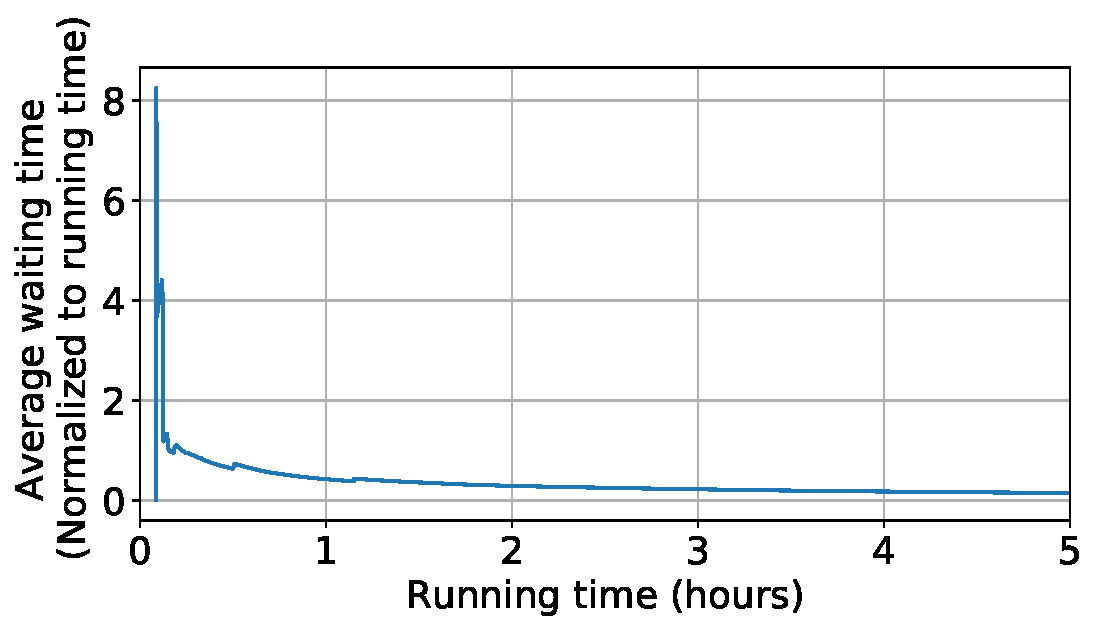
\includegraphics[width=0.4\textwidth]{../data/waiting_cumul.pdf}
%   \caption{The average waiting time (normalized to running time) of jobs of different length.}
%   \label{fig:hpc-wait-cdf}
% \end{figure}



%%% Local Variables:
%%% mode: latex
%%% TeX-master: "paper"
%%% End:


\vspace*{\subsecspace}
\section{Related Work}
\label{sec:related}


\sysname builds upon a large body of prior work on running scientific computing applications on the cloud, and the various facets of transient cloud computing.  

\vspace*{\subsecspace}
\subsection{Cloud Computing For Science}
Running scientific applications on the cloud introduces many tradeoffs compared to conventional HPC clusters, along the dimensions of performance, cost, scalability, convenience, and reproducability.
These tradeoffs are explored in~\cite{iosup_performance_2011, zhai_cloud_2011, marathe2013comparative, galante_analysis_2016, benedictis_cloud-aware_2014}.
In general, clouds can provide increased elasticity, lower waiting times, and more choices in resource allocation that can be tailored to the application.
The cloud resource model is also present in platforms like nanoHUB~\cite{nanohub}, that provide easy execution and dissemination of nanotechnology simulation applications.
%such as Ref.~\cite{kadupitiya2017}.
Outside of the bags of jobs execution model, price optimizations for scientific workflows in the cloud is discussed in~\cite{gari_learning_2019}. 
While bags of tasks~\cite{varshney_autobot_2019} are often used for parallel applications, \sysname is the first to use the bags of \emph{jobs} abstraction for efficient and effective use of transient servers. 

%\subsubsection{Bags of Jobs}
\vspace*{\subsecspace}
\subsection{Transient Cloud Computing}

%The low cost of transient cloud servers has made them very appealing, inspite of their preemptible nature, and their efficient and effective use has been a significant amount of research~\cite{prateek-thesis}. 
The challenges posed by Amazon EC2 spot instances, the first transient cloud servers, have received significant attention from both academia  and industry~\cite{spotinst}. 
Since spot instances are significantly cheaper than the equivalent on-demand servers, they are attractive for running preemption and delay tolerant batch jobs~\cite{spoton, jain14demand, yi2010reducing, conductor, liu-spot, spot-run, dubois2016optispot}.
A crucial component of EC2 spot instances is their dynamic auction-based pricing, and choosing the ``right'' bid price to minimize cost and performance degradation is the focus of much of the past work on transient computing~\cite{bidding4,mihailescu2012impact,bidding7,bidding1,bidding8,bidding3,bidding6,bid-cloud,bidding5,wolski_probabilistic_2017, guo_bidding_2015}.
However, as explained in Section~\ref{subsec:need-for-empirical}, it remains to be seen how Amazon's recent change~\cite{bid-change} in the preemption model of spot instances affects prior work.


On the other hand, the effective use of transient resources provided by other cloud providers such as Google, Microsoft, Packet, and Alibaba largely remains unexplored. 
Ours is the first work that studies the preemption characteristics and addresses the challenges involved in running large-scale applications on the Google Preemptible VMs, and provides insights on the unique preemption dynamics, as explained in Section~\ref{sec:preemption-dynamics}.

\vspace*{\subsecspace}
\subsubsection{Preemption Mitigation}
Effective use of transient servers usually entails the use of fault-tolerance techniques such as checkpointing~\cite{flint}, migration~\cite{spotcheck}, and replication.
In the context of HPC workloads,~\cite{marathe2014exploiting,gong_monetary_2015,xiang_spotmpi:_2011} develop checkpointing and bidding strategies for MPI applications running on EC2 spot instances, based on older spot pricing models. 
%, which are inherently memoryless and not applicable in our case. 
Periodic checkpointing~\cite{dongarra_fault_nodate} is not appropriate in our case because preemptions are not memoryless. 

By treating bags of jobs as an execution unit, allowing some jobs to fail, and using insights from preemption models, we show that it is possible to reduce the recomputation times to acceptable levels even without the  use of periodic  checkpointing that imposes additional deployment and performance overheads. 
%The first step towards mitigating preemptions is understanding their characteristics. 
Our preemption model for Google preemptible VMs developed in Section~\ref{sec:preemption-dynamics} provides a novel characterization of bathtub shaped failure rates not captured by the classic Weibull distribution, and is distinct from prior efforts~\cite{mudholkar1993exponentiated, crevecoeur1993model}. 

%extends the classic Weibull-distribution based bathtub models~\cite{mudholkar1993exponentiated, crevecoeur1993model} by introducing exponential reclamation near the deadline and additional paramters that capture and explain the preemption dynamics. 

\vspace*{\subsecspace}
\subsubsection{Server Selection}

Optimized server selection is an important problem in cloud computing, and especially for transient servers because of the cost-performance-preemption tradeoff involved. 
Similar to \sysname, SpotOn~\cite{spoton} is also a batch computing service that selects servers based on job characteristics and failure rates of different EC2 spot VMs. However, it is restricted to individual, single-VM batch jobs, and its design is tied to EC2 spot instances.
The state of the art transient server selection involves the use of multiple types of VMs~\cite{exosphere}, and selecting a heterogeneous cluster can reduce the likelihood of mass concurrent preemptions.
However, since scientific computing applications are mostly synchronous, even a single failure affects the entire job, and heterogeneous clusters are not required, and are in fact, detrimental~\cite{exosphere}. 
Server selection is important even outside of preemptible VMs---developing bayesian optimization and application performance model based search for the ``best'' cloud VM is an active research area~\cite{alipourfard_cherrypick, yadwadkar_selecting_2017}, but these techniques do not  account  for preemptions. 

\begin{figure}[t]
  \centering 
       \vspace*{\myfigspace} 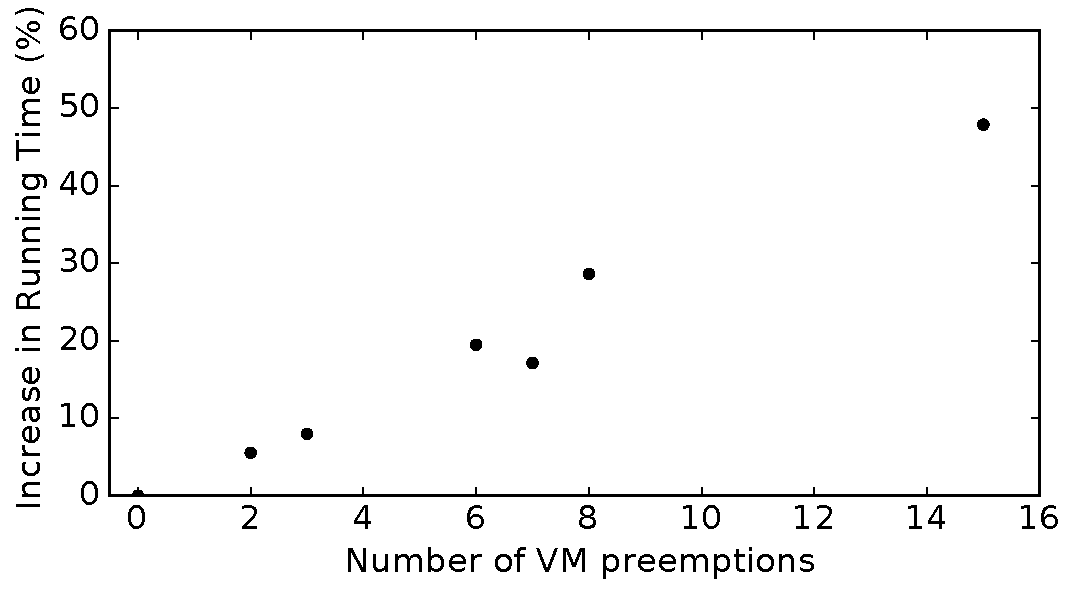
\includegraphics[width=0.22\textwidth]{../graphs/confin-fails-vs-time-relative.pdf}
      \vspace*{\myfigspace}
  \caption{The increase in running time due to preemptions is under 50\%, even when the number of preemptions is high.}
  \label{fig:fails-time}
        \vspace*{\myfigspace}
\end{figure}




\vspace*{\subsecspace}
%Parameter sweep aka bags of jobs ~\cite{casanova_heuristics_2000}

%But nothing for bags of jobs themselves.. 


% \subsubsection{Fault-tolerance}

% All the past work was on EC2 spot market with gang failures and independent markets~\cite{marathe2014exploiting, gong_monetary_2015}.
% However this assumption has now changed, and failures can happen anytime.
% Our failure model is more general, and applies to both cases.



% \cite{dongarra_fault_nodate} has a discussion of checkpointing frequency which is comprehensive. Replication is another way~\cite{walters_replication-based_2009}

% Non periodic checkpointing~\cite{bougeret_checkpointing_2011}


% \subsubsection{Failure Modeling}



% Crevecour etc. 



% \subsubsection{Server Selection}
% Exploring a large configuration space using bayesian optimization methods in CherryPick~\cite{alipourfard_cherrypick} and Metis~\cite{li2018metis}.

% Can also use Latin Hypercube sampling for parameter exploration?




%%% Local Variables:
%%% mode: latex
%%% TeX-master: "paper"
%%% End:


\vspace*{\subsecspace}
\section{Discussion and Future Directions}
\label{sec:discussion}

% We have made an initial exploration into constrained preemptions, and many questions remain to be answered.
% Below, we discuss some aspects of pertaining to our model and avenues for future investigation.

Constrained preemptions are a relatively unexplored phenomenon and challenging to model.
Our model and the associated data expand transient cloud computing to beyond EC2-spot.
We have evaluated the model under different practical conditions including different VM types and temporal domains, and have shown it to be general and robust. 
However, many questions and avenues of future investigation remain open:

\noindent \textbf{What if preemption characteristics change?}
%Ultimately, the preemption characteristics are based on the cloud provider policies, the supply and demand of transient and on-demand and reserved VMs, etc., and may change over time.  
Our model allows detecting policy and phase changes by comparing observed data with model-predictions and detect change-points, and 
a long-running cloud service can continuously update the model based on recent preemption behavior. 
However, changes are rare: Google's preemption policy has not changed since its inception in 2015. 
%EC2 pricing and preemptions were relatively stable~\cite{hotcloud-not-bid} until 2017~\cite{irwin-icccn19, baughman2019deconstructing, spotweb}.
%
Regardless, VMs with constrained preemptions are an interesting \emph{new} type of transient resource, and our analysis, observations, and policies should continue to be relevant. 
Furthermore, we demonstrate that the multi-phase bathtub failure distribution may be a fundamental characteristic of constrained preemptions that benefit both the cloud platform and applications, and thus models that capture the distinct preemption phases would still be relevant even if the finer-grained preemption characteristics change. % over time. 
%
We have also shown that our policies are not particularly sensitive to the model parameters, and even using a ``wrong'' or outdated model can provide significant benefits compared to existing memoryless models. 

\noindent \textbf{\emph{Phase-wise} model.}
Our statistical analysis indicates that the preemption rates have three distinct phases. 
%Our model is a continuously differentiable and allows capturing the three phases reasonably well. 
\vikram{The analytical model derived in this work is continuously differentiable and allows capturing the three phases reasonably well.}
It may be possible to use a ``phase-wise'' model such as a piece-wise continuously differentiable model, where the three phases are modeled either as segmented linear regions (found using segmented linear regression), or an initial exponential phase and two linear phases. 
Such a piece-wise model could capture the phase transitions with even more accuracy.
\vikram{Further, one may consider the use of such models (heurestics) as preferred for their simplicity. However the analytical form for the predictive model enables for a cleaner integration with the resource management service. The analytical form for the preemption distributions as well as the rates can also be used to distill contributions of distinct phases in a more convenient manner. It also provides a measure to distill the contirbutions of the discontinuties present in the real operation (which are coarse-grained over in the continuously differentiable model) in changing the VM expected lifetimes and checkpointing policies. From the other end, there is a prevalent use of analytical models to extract information from preemption data (EC2). Our intent is to provide an analogous minimal model for the Google preemptible instances that can then be used to compare with existing analytical models on the same footing (as opposed to comparing simple heurestics in one with analytical forms in the other). This paper addresses the need for a minimal analytical model to describe non-memoryless preemptions, and we expect this to not inhibit the development of simpler empirical modeling approaches, but guide such model development with a fully-parameterized analytical model based on sound first principles and well-defined assumptions.
}

\begin{comment}
\noindent \textbf{Connection to constrained systems and statistical mechanics.} Our proof of Lemma~\ref{lemma:1} used mapping to constrained physical systems and employed the statistical mechanics tools such as partition functions \cite{krauth2006statistical}. 
We have only presented the initial connection between the behavior of constrained preemptions and the statistical mechanics of constraint-driven phenomena in many particle systems \cite{krauth2006statistical,solis}, and we conjecture that a deeper analogy may exist. 
Central to our proof is the assumption of mutually exclusive preemptions---that is, the provider preempts VMs in a mutually exclusive manner.
This assumption makes sense from a cluster management and application perspective. 
However, analyzing constrained preemptions with weaker versions of the mutual exclusion assumption is \emph{also} possible with statistical mechanics approaches. 
For example, for studies of situations where weakly overlapping preemptions are preferred, one can leverage the statistical mechanics framework of constrained ``soft'' particles often investigated using molecular dynamics simulations \cite{jing2015ionic}.
\end{comment}

%where mutual exclusion is only preferred and not mandatory, we can leverage the statistical mechanics of constrained ``soft'' particles, which is also a well studied \cite{solis}, often with molecular dynamics simulations \cite{jyto}. 

%%% Local Variables:
%%% mode: latex
%%% TeX-master: "paper"
%%% End:




\section{Conclusion}
\label{sec:conclusion}
The effective use of transient computing relies on understanding the preemption characteristics.
While past work on transient computing has developed techniques and systems for Amazon's EC2 spot instances, ours is the \emph{first} work to understand the behavior of Google's Preemptible VMs, that have a unique characteristic of having a maximum 24 hour lifetime.
Our large-scale empirical study shows that the constraint imposes a bathtub failure distribution, and we develop a new phenomenological probability model for capturing its three distinct temporal phases. 
Our insights and model-based policies can reduce the preemption overheads by more than $5\times$ compared to existing preemption models, and our batch computing service can reduce computing costs by over $5\times$. 



%%% Local Variables:
%%% mode: latex
%%% TeX-master: "paper"
%%% End:


%% 10 pages plus references 
%\clearpage 

{
\bibliographystyle{acm}
\interlinepenalty=10000 %%%%For fixing url-related errors only 
\bibliography{scicloud,bagsjobs,spot-bid}
%\bibliography{bagsjobs}
}


\end{document}


%%% Local Variables:
%%% mode: latex
%%% TeX-master: t
%%% End:
